\documentclass[]{book}
\usepackage{lmodern}
\usepackage{amssymb,amsmath}
\usepackage{ifxetex,ifluatex}
\usepackage{fixltx2e} % provides \textsubscript
\ifnum 0\ifxetex 1\fi\ifluatex 1\fi=0 % if pdftex
  \usepackage[T1]{fontenc}
  \usepackage[utf8]{inputenc}
  \usepackage{eurosym}
\else % if luatex or xelatex
  \ifxetex
    \usepackage{mathspec}
  \else
    \usepackage{fontspec}
  \fi
  \defaultfontfeatures{Ligatures=TeX,Scale=MatchLowercase}
  \newcommand{\euro}{€}
\fi
% use upquote if available, for straight quotes in verbatim environments
\IfFileExists{upquote.sty}{\usepackage{upquote}}{}
% use microtype if available
\IfFileExists{microtype.sty}{%
\usepackage{microtype}
\UseMicrotypeSet[protrusion]{basicmath} % disable protrusion for tt fonts
}{}
\usepackage[unicode=true]{hyperref}
\hypersetup{
            pdftitle={A Clinical Trials Toolkit},
            pdfauthor={The Interventional Studies in Aging Center at IFAR},
            pdfborder={0 0 0},
            breaklinks=true}
\urlstyle{same}  % don't use monospace font for urls
\usepackage{longtable,booktabs}
% Fix footnotes in tables (requires footnote package)
\IfFileExists{footnote.sty}{\usepackage{footnote}\makesavenoteenv{long table}}{}
\usepackage{graphicx,grffile}
\makeatletter
\def\maxwidth{\ifdim\Gin@nat@width>\linewidth\linewidth\else\Gin@nat@width\fi}
\def\maxheight{\ifdim\Gin@nat@height>\textheight\textheight\else\Gin@nat@height\fi}
\makeatother
% Scale images if necessary, so that they will not overflow the page
% margins by default, and it is still possible to overwrite the defaults
% using explicit options in \includegraphics[width, height, ...]{}
\setkeys{Gin}{width=\maxwidth,height=\maxheight,keepaspectratio}
\IfFileExists{parskip.sty}{%
\usepackage{parskip}
}{% else
\setlength{\parindent}{0pt}
\setlength{\parskip}{6pt plus 2pt minus 1pt}
}
\setlength{\emergencystretch}{3em}  % prevent overfull lines
\providecommand{\tightlist}{%
  \setlength{\itemsep}{0pt}\setlength{\parskip}{0pt}}
\setcounter{secnumdepth}{5}
% % Redefines (sub)paragraphs to behave more like sections
% \ifx\paragraph\undefined\else
% \let\oldparagraph\paragraph
% \renewcommand{\paragraph}[1]{\oldparagraph{#1}\mbox{}}
% \fi
% \ifx\subparagraph\undefined\else
% \let\oldsubparagraph\subparagraph
% \renewcommand{\subparagraph}[1]{\oldsubparagraph{#1}\mbox{}}
% \fi
% 
% set default figure placement to htbp
\makeatletter
\def\fps@figure{htbp}
\makeatother

%%%%%%%%%%%%%%%%%%%%%% Customized tgt 2014.12.16 %%%%%%%%%%%

%% document formatting
\usepackage{tabularx,tabulary}
\usepackage{tabu}

%% fonts setup

\usepackage{fontspec}
\usepackage{xunicode} %xelatex access to accents, etc
\usepackage{xltxtra}
\usepackage{unicode-math}
\usepackage{gensymb} %degree symbol

\setmainfont[Mapping=tex?text, Numbers={Proportional, OldStyle}, Ligatures=TeX]{Linux Libertine O}
\setsansfont[Mapping=tex?text, Numbers={Proportional, OldStyle}, Ligatures=TeX]{Linux Biolinum O}
\setmathfont{Asana Math}

% \usepackage{microtype}
% \usepackage{float} % used to fix floating objects to a specific spot

%% tables and figures

\usepackage{array} % for dealing with table spacing
\usepackage[flushleft]{threeparttablex} % tables with caption, content, footnotes; captions and footnotes the same width as table body (wrapping)
\usepackage{makecell} % allow linebreaks in table cells using \thead (headers) and \makecell
\usepackage{etoolbox}
\robustify\tnote

\usepackage{titlesec}

\usepackage{booktabs, dcolumn, float, microtype} % formatted tables, decimal alignment, dealing with floats, title and section formatting
\usepackage[usenames,dvipsnames,svgnames,table]{xcolor} % colors for tables and text

\newcommand{\head}[1]{% column header environment
  {\small \setstretch{.85} \begin{tabular}[c]{ @{}c@{}}
  #1
  \end{tabular}}%
}

\setlength{\tabcolsep}{4.5pt} % space between table columns
 \renewcommand{\arraystretch}{1.5} % space between table rows
%\setlength{\extrarowheight}{10pt}

% table/figure captions (titles and legends)
\usepackage{caption}
\DeclareCaptionFormat{llap}{\llap{#1#2}#3\par} % table / figure number in left margin
\DeclareCaptionLabelSeparator{spc}{\hspace{.075 in}} % space between table number and caption
\captionsetup{font={color=blue, sf}, singlelinecheck=off, margin= 15pt, skip=4pt, size=small, labelfont={sc, sf}, format=llap, labelsep=spc,singlelinecheck=no} % same font as headers

% non-table footnotes
\usepackage[hang]{footmisc}

% [para,online,flushleft]

% headers and footers

%% section headings font and spacing
 %\usepackage{titlesec}
 \usepackage{titling}

\newfontfamily\headingfont[]{Linux Biolinum O}
 \titleformat*{\section}{\sc \large \color[rgb]{0,0,0} \headingfont}
 \titleformat*{\subsection}{\large \headingfont}
 \titleformat*{\subsubsection}{\normalsize \headingfont}
 \renewcommand{\maketitlehooka}{\headingfont}

 \titlespacing*{\section}{0pt}{8pt plus 2pt minus 2pt}{0pt plus 2pt minus 2pt}
 \titlespacing*{\subsection}{0pt}{6pt plus 2pt minus 2pt}{-2pt plus 2pt minus 2pt}
 \titlespacing*{\subsubsection}{0pt}{2pt plus 2pt minus 2pt}{-3pt plus 2pt minus 2pt}

%% definition and spacing of section numbers

% put section numbers in margin
\makeatletter
\def\@seccntformat#1{\llap{\csname the#1\endcsname \hspace{.075 in}}}
\makeatother

% spacing of bulleted lists
\usepackage{enumitem} %control spacing of enumerated items
\setlist[itemize]{noitemsep, topsep=0pt}

% -------------------------


\usepackage{tikz}

% table decimal alignment
\usepackage[detect-all]{siunitx}
\sisetup{table-format = 3.3, input-symbols = >()<, tight-spacing = true, table-space-text-pre = $<$} % table-align-text-post = false,

\newlength\tbspace
\setlength\tbspace{.25in}
\newcolumntype{T}{S<{\hspace{\tbspace}}}
\newcolumntype{C}{c<{\hspace{\tbspace}}}


\newcolumntype{d}{D{.}{.}{-1}} % decimal justify table contents
\newcolumntype{z}[1]{>{\centering\let\newline\\\arraybackslash\hspace{0pt}}p{#1}}


% units.
\usepackage{units}

% graphix
\usepackage{graphicx}
\setkeys{Gin}{width=\linewidth,totalheight=\textheight,keepaspectratio}

\title{A Clinical Trials Toolkit}
\author{The Interventional Studies in Aging Center at IFAR}
\date{}

\begin{document}
\maketitle

{
\setcounter{tocdepth}{1}
\tableofcontents
}
\clearpage 

\chapter{Introduction}\label{introduction}

\section{Purpose of this toolkit}\label{purpose-of-this-toolkit}

This toolkit is a \emph{general} guide for investigators and project
staff at Hebrew SeniorLife Institute for Aging Research (HSL IFAR)
conducting, managing or overseeing clinical trials in older populations.
The toolkit is not intended be a comprehensive document. Rather it is
meant to outline major considerations for all phases of a clinical
trial. Suggested resources are provided for more detailed information
\textbf{and you must consult and adhere to the latest federal, sponsor,
institutional, state and regional regulations.}

Whenever possible, sections of this toolkit follow a similar outline:
What, Why, How, Special Considerations for Aging Populations, Common
Pitfalls, and Resources.

\section{Are you are doing a clinical
trial?}\label{are-you-are-doing-a-clinical-trial}

Below is the National Institutes of Health (NIH) definition of a
clinical trial. As clinical trials are subject to additional oversight,
a clear definition helps investigators ensure that they are meeting all
of their obligations, and help funders ensure that the additional
oversight is occurring when it is needed.

\begin{quote}
A research study\textsuperscript{1~}in which one or more human
subjects\textsuperscript{2}~are prospectively
assigned\textsuperscript{3}~to one or more
interventions\textsuperscript{4}~(which may include placebo or other
control) to evaluate the effects of those interventions on
health-related biomedical or behavioral outcomes.\textsuperscript{5}
\end{quote}

\emph{\textsuperscript{1}See Common Rule definition of }research* at 45
CFR 46.102(d).*

\emph{\textsuperscript{2}See Common Rule definition of }human subject*
at 45 CFR 46.102(f).*

\emph{\textsuperscript{3}``Prospectively assigned'' refers to a
pre-defined process (e.g., randomization) specified in a protocol that
stipulates the assignment of research subjects (individually or in
clusters) to one or more arms of a clinical trial.}

\emph{\textsuperscript{4}An~intervention~is defined as a manipulation of
the subject or subject's environment for the purpose of modifying one or
more health-related biomedical or behavioral processes and/or
endpoints.~ Examples include:~ drugs/small molecules/compounds;
biologics; devices; procedures (e.g., surgical techniques); delivery
systems (e.g., telemedicine); strategies to change health-related
behavior (e.g., diet, cognitive therapy, exercise); treatment
strategies; prevention strategies; and, diagnostic strategies.}

\emph{\textsuperscript{5}Health-related biomedical or behavioral
outcome~is defined as the pre-specified goal(s) or condition(s) that
reflect the effect of one or more interventions on human subjects'
biomedical or behavioral status or quality of life.~ Examples include:~
positive or negative changes to physiological or biological parameters
(e.g., improvement of lung capacity); positive or negative changes to
psychological or neurodevelopmental parameters (e.g., mood management
intervention for smokers; reading comprehension and /or information
retention); positive or negative changes to disease processes; positive
or negative changes to health-related behaviors; and, positive or
negative changes to quality of life.}

\href{https://grants.nih.go\%20v/grants/guide/notice-files/NOT-OD-15-015.html}{https://grants.nih.go
v/grants/guide/notice-files/NOT-OD-15-015.html}

\section{Clinical Trial Phases}\label{clinical-trial-phases}

Clinical trials are conducted in a series of steps, called phases - each
phase is designed to answer a separate research question. These phases
mostly apply to trials testing drugs or devices, rather than behavioral
interventions.

\begin{itemize}
\item
  \textbf{Phase I:}~Researchers test a new drug or treatment in a small
  group of people for the first time to evaluate its safety, determine a
  safe dosage range, and identify side effects.
\item
  \textbf{Phase II:}~The drug or treatment is given to a larger group of
  people to see if it is effective and to further evaluate its safety.
\item
  \textbf{Phase III:}~The drug or treatment is given to large groups of
  people to confirm its effectiveness, monitor side effects, compare it
  to commonly used treatments, and collect information that will allow
  the drug or treatment to be used safely.
\item
  \textbf{Phase IV:}~Studies are done after the drug or treatment has
  been marketed to gather information on the drug's/treatment's effect
  in various populations and any side effects associated with long-term
  use.
\end{itemize}

\section{Training requirements and
opportunities:}\label{training-requirements-and-opportunities}

Aside from clinical trial design and/or biostatistical training, there
are varied practical, short-term courses for principal investigators and
project personnel to enhance the conduct and rigor of their clinical
trials.

\begin{enumerate}
\def\labelenumi{\arabic{enumi}.}
\item
  \textbf{Good Clinical Practice}~(\textbf{GCP}) is an international
  quality standard that defines standards for clinical trials involving
  human subjects. \textbf{The NIH require
  C}\href{http://grants.nih.gov/grants/guide/notice-files/NOT-OD-16-148.html\#_ftn2}{\textbf{ertifications
  in Good Clinical Practice}} \textbf{for NIH-funded Investigators and
  clinical trial site staff who are responsible for the conduct,
  management and oversight of NIH-funded clinical trials. The FDA has a
  similar requirement.} Below is a link to its training that fulfils
  this requirement:
  \url{https://gcplearningcenter.niaid.nih.gov/Pages/default.aspx}

  There are many other extensive courses offered to become GCP
  certified, both internet-based and on-site. Most have a tuition cost.
  It is a good idea, if resources are available, for Project Directors
  leading clinical trials to receive GCP certification. Below are
  examples of a few of these many opportunities.

  \url{https://gcp.nihtraining.com/}

  \url{http://www.onlinegcp.us/}

  \url{https://www.citiprogram.org/index.cfm?pageID=90}
\item
  \textbf{Harvard Catalyst Clinical Trial Design:} Clinical Trial Design
  is an opportunity for new clinical investigators, who have an idea for
  development of a clinical trial, to participate in an intensive
  eight-week course. It is offered at \emph{no cost} to members of the
  Harvard Catalyst community or other Clinical and Translational Science
  Award(CTSA) usually in May/June, with an application due in March.
  Participants learn the fundamentals of clinical trial design,
  including instructions on how to design a protocol, information on IRB
  and regulatory topics, and on trial implementation. Additional course
  topics include statistical analysis, budgeting, and data management.
  \url{https://catalyst.harvard.edu/services/ctd/}
\item
  \textbf{NIH Clinical Research Training On-Line:} On-line course
  available 24/day at no cost with the following objectives: i. To raise
  awareness of the ethical issues involved in human subjects research;
  ii. To become familiar with the roles and responsibilities of the
  principal investigator and the institution when conducting clinical
  research in the NIH intramural research program; iii. To have an
  understanding of Food and Drug Administration (FDA) oversight of
  clinical research; and iv. To become familiar with how developments in
  science and health are reported by the media and how to work
  effectively with reporters.

  \href{http://crt.nihtraining.com/}{http://crt.nihtraining.com}
\item
  \textbf{Barnett International: Design and Conduct of Clinical Trials:
  Design Requirements, Statistical Issues, and Clinical Protocols:}
  On-site two-day course that provides an introduction to the
  scientific, statistical, and ethical aspects of clinical trials
  research.~Cost (2016) = \$1800

  \url{http://www.barnettinternational.com/Live-Seminars/Design-and-Conduct-of-Clinical-Trials--Design-Requirements,-Statistical-Issues,-and-Clinical-Protocols/}
\end{enumerate}

\section{Clinical Trial Planning
Resources}\label{clinical-trial-planning-resources}

Numerous resources are available to researchers as they plan and proceed
with their clinical trial.

\begin{enumerate}
\def\labelenumi{\arabic{enumi}.}
\tightlist
\item
  One such resources is **``The NIA Clinical Trial Toolbox: A resource
  for quality studies**
  (\url{https://www.nia.nih.gov/research/blog/2016/10/nia-clinical-trial-toolbox-resource-quality-studies}).
  This toolbox provides researchers with a central source of materials
  to develop and manage clinical trials. The site includes: templates,
  forms, guidelines and other related information that can be very
  helpful throughout the research process and is referenced throughout
  the ISAC toolkit
\end{enumerate}

\chapter{Experimental Design and Statistical
Considerations}\label{experimental-design-and-statistical-considerations}

\section{Introduction}\label{introduction-1}

\subsection{What}\label{what}

Experimental design encompasses features of a clinical trial that relate
to its structure and operations.

\subsection{Why}\label{why}

Careful planning and documentation of design of a clinical intervention
study is critical for maintenance of rigor and the obtaining of results
that are likely to be reproducible. These considerations are intimately
connected to the trial's appropriateness for formal statistical analysis
and production of results. It is thus imperative that all aspects of
design receive the highest level of scrutiny during the planning phase.

\subsection{How}\label{how}

It is critical that aspects of design be tailored to the goals and
specific aims of the trial. Below we delineate aspects of experimental
and statistical design that should be considered. These are not to be
considered comprehensive or as being equally applicable to all
scenarios, but should provide a starting point in planning your study.

\section{Design of the study}\label{design-of-the-study}

\subsection{What}\label{what-1}

In this toolkit we consider explicitly randomized experiments conducted
with human subjects, most typically clinical trials.

\subsection{Why}\label{why-1}

Key design features will ultimately dictate the internal validity and
generalizability of trial results.

\subsection{How}\label{how-1}

The following items should be considered during the design phase.

\begin{enumerate}
\def\labelenumi{\arabic{enumi}.}
\tightlist
\item
  Rationale for conduct of the trial. \emph{The scientific / biomedical
  impetus necessitating conduct of the trial}
\item
  Overall goal. \emph{What, specifically, the study is intended to
  accomplish. Investigators should note the degree to which the trial
  will be considered \textbf{explanatory} (that is, focused on
  estimation of pure causal effects of intervention under controlled
  circumstances) versus \textbf{pragmatic} (focused on choosing between
  therapeutic options, often under circumstances mimicing or derived
  directly from clinical experience.) Many studies will have both
  explanatory and pragmatic aims.}
\item
  Illness condition or state. \emph{The condition modification of which
  motivates the study.}
\item
  Sampling population. \emph{Individuals on whom sampling should focus,
  including explicit requirements for inclusion and factors that would
  preclude enrollment (exclusions).}
\item
  General approach to design. \_Determination of the general nature of
  the approach to determining intervention efficacy and safety. For
  instance, the trial may be intended to demonstrate
  \textbf{superiority,} \textbf{noninferiority} or \textbf{equivalence}
  of a novel intervention to standard care; to determine \textbf{maximum
  tolerable dose} of a particular agent in a given population; to
  demonstrate a \textbf{dose-response} relation between intervention
  dosing and endpoints; etc.
\item
  Specific aims. \emph{Detailed aims addressable by evaluation of
  statistical hypotheses.}
\item
  Primary and secondary endpoints.
\item
  General nature of the planned comparisons. \emph{Key features of the
  comparisons to be made; e.g.~mean performance on a primary endpoint.}
\item
  Safety concerns. \emph{Risks, including loss of confidentiality,
  affiliated with intervention or trial activities. Note that these will
  be explicitly considered by Institutional Review Board in assessing
  the risk/benefit ratio of conduct of the trial.}
\item
  Ethical considerations. \emph{Additional safety of ethical
  considerations}
\item
  Measurement and quantification of effects. \emph{The way in which
  treatment effects will be quantified.}
\item
  Determination of statistical significance of comparisons.
  \emph{Summary nature of quantitative comparisons, fleshed out in
  statistical analysis plan}
\item
  Study staffing and environment

  \begin{enumerate}
  \def\labelenumii{\roman{enumii}.}
  \tightlist
  \item
    Leadership. \emph{Designation of membership and roles of
    investigative team leaders.}
  \item
    Staffing. \emph{Designation of study staff, with specific
    delineation of responsibilities.}
  \item
    Environment. \emph{Physical space in which the study will be
    conducted. Explicitly considers access and travel to and from the
    venue, as appropriate.}
  \end{enumerate}
\item
  Measurement \emph{Detailed explication of the was in which
  measurements will be taken. Makes specific note of resource needs (for
  instance, whether images or biospecimens must be collected or stored,
  and the equipment, facilities and human resources necessray to obtain
  said measures.)}
\item
  Nature and administration of intervention \emph{Specific detail on the
  intervention, including how, how frequently, and by whom it will be
  administered and monitored}
\item
  Study intervention period \emph{Length of time over which intervention
  would be administered, including run-in and washout periods as
  applicable}
\item
  Frequency of participant interactions, data collection and endpoint
  measurement \emph{Number and frequency of participant interactions and
  measurments; often displayed in tabular format}
\item
  Participant allocation or randomization \emph{Methods by which
  participants will be assigned to trial arms, e.g.~by randomization.
  Detail on the specific procedures used to determine these assignments.
  Must consider factors (e.g.~blocking or stratification) that affect
  this process.}
\item
  Masking / blinding \emph{Determination of whether and how
  investigators, staff, participants, analysts etc. are aware of
  intervention assignments.}
\item
  Data collection and management \emph{Detail on the physical systems
  for data capture, methods by which it will be captured, the persons
  performing entry, monitoring of data completeness and quality, etc.
  See Data Management module}.
\item
  Statistical design and sample size \emph{See below}
\item
  Measurement of trial adherence \emph{Methods by which completeness of
  planned participant interactions with randomized activities will be
  quantified, and plans for analysis, if any}
\item
  Training \emph{Provisions for training of study personnel, including
  human resources for providing the trainging}
\end{enumerate}

\subsection{Special considerations for older
adults}\label{special-considerations-for-older-adults}

The number of participants available and who would likely consent to be
enrolled in trials can be difficult to estimate among older individuals,
particularly in the context of numerous exclusionary factors.

\subsection{Common pitfalls}\label{common-pitfalls}

Lack of specificity in describing intervention; insufficient attention
to the potential for attrition, data missingness, or intervention
non-adherence; lack of detail in considering manner by which
participants may be contacted, recruited, and maintained in the trial.

\subsection{Resources}\label{resources}

\section{General Statistical
Considerations}\label{general-statistical-considerations}

\subsection{What}\label{what-2}

The statistical design works hand-in-hand with the experimental design
to establish procedures for data interpretation and analysis. Major
considerations include planning the enrollment and sample size, the
general analytic approach, a priori consideration of the way in which
results will be interpreted, and plans to resolve expected and
unexpected problems, including data missingness and untoward
measurements.

\subsection{Why}\label{why-2}

Appropriate sample size and a statistical analysis plan are critical for
the validity of conclusions and to prevent bias in operations and
conclusions.

\subsection{How}\label{how-2}

Derivation of the statistical analysis plan is detailed in the sections
below.

\hypertarget{statistical-analysis-plan}{\section{Statistical Analysis
Plan}\label{statistical-analysis-plan}}

\subsection{What}\label{what-3}

The project Statistical Analysis Plan (\textbf{SAP}) provides
\textbf{detailed} descriptions of statistical analyses to be conducted
for the trial, including rationale for choice of methods, plans for
dealing with unexpected difficulties, and pre-specified guidance on
interpretation of results.

\subsection{Why}\label{why-3}

Guidance on data ascertainment, management, storage, analysis and
interpretation are critical to preserve the validity of the design and
soundness of scientific conclusions.

\subsection{How}\label{how-3}

A version of the SAP may be included as an addendum to or embedded
within the study protocol and manual of procedures, but ideally the
authoritative SAP should be an independent document with its own
formatting, references etc. The SAP must be assembled prior to
enrollment and approved by the appropriate parties including the trial
statistician, investigative team, and regulatory authorities
(e.g.~DSMB), and may be included with the package submitted to
Institutional Review Boards or equivalent overseeing ethical approval of
the trial. Authorship should be by the project statistician, assisted by
the investigative team. As with all trials documents, the SAP should be
under strict version control, and a `living' electronic date-stamped
version considered the authoritative document (see \textbf{Essential
Documents} ).

\subsubsection{Contents of the document}\label{contents-of-the-document}

The contents of the SAP will vary from trial to trial. For a
conventional intervention trial designed to assess efficacy, in which
participants are allocated to one of two or more groups
(e.g.~intervention vs.~control), contents might be as follows.

\begin{enumerate}
\def\labelenumi{\arabic{enumi}.}
\tightlist
\item
  Introduction

  \begin{enumerate}
  \def\labelenumii{\alph{enumii}.}
  \tightlist
  \item
    Background. \emph{Provides explanatory information concerning
    disease target, patient population, etc. Includes references to
    authoritative literature.}
  \item
    Objectives. \emph{Briefly describes overall analytic goals.}

    \begin{enumerate}
    \def\labelenumiii{\roman{enumiii}.}
    \tightlist
    \item
      Primary objective. \emph{Describes primary objective of the trial,
      being specific concerning such matters as demonstration of
      feasibility; efficacy / effectiveness; safety. Provides some
      clarity concerning expected treatment effects and public health
      relevance.}
    \item
      Secondary objectives. \emph{As above, for secondary objectives.}
    \end{enumerate}
  \end{enumerate}
\item
  Endpoints

  \begin{enumerate}
  \def\labelenumii{\alph{enumii}.}
  \tightlist
  \item
    Primary endpoints. \emph{Describes primary and secondary endpoints.
    May give detail as to measurement, validity and reliability, and
    other performance characteristics.}
  \item
    Secondary endpoints. \emph{As above, for secondary endpoints.}
  \end{enumerate}
\item
  Protocol / Grant SAP. \emph{Summarize existing plan as presented in
  the original protocol or funding application.}\\
\item
  Design elements

  \begin{enumerate}
  \def\labelenumii{\alph{enumii}.}
  \tightlist
  \item
    Basic design features. \emph{Discusses overall experimental
    structure for purposes of comparison.}

    \begin{enumerate}
    \def\labelenumiii{\roman{enumiii}.}
    \tightlist
    \item
      Nature of primary comparison. \emph{Describes the basic target of
      interest, i.e.~determination of superiority, equivalence or
      noninferiority of intervention to control or current standard of
      care.}
    \item
      Participant allocation. \emph{Describes randomization or other
      procedures by which participants are allocated to trial groups.}
    \end{enumerate}
  \item
    Schedule of events. \emph{Gives a summary of time-points and
    measurements that will be used.}
  \item
    Blinding. \emph{Describes the degree to which data scientists and
    personnel are blinded, and maintenance of same.}
  \item
    Blocking and stratification / matching. \emph{Describes blocking,
    matching, etc. and references plans for consideration of design
    effects in analysis.}
  \item
    Randomization Scheme. \emph{Describes the randomization scheme and
    procedures.}
  \item
    Intended Sample Size. \emph{Describes the intended final sample
    size, referencing potential hurdles such as attrition, crossover,
    non-adherence and other sources of bias.}
  \item
    Effects intended to be estimated. \emph{Describes inferential
    targets for the analysis.}

    \begin{enumerate}
    \def\labelenumiii{\roman{enumiii}.}
    \tightlist
    \item
      Bounds for determination of statistical significance. \emph{Gives
      clinical and statistical thresholds for determination of
      significance of evidence and, where appropriate, rejection of null
      hypotheses.}
    \item
      Argument for clinical significance ) \emph{Establishes clinical
      relevance of effect to be estimated, potentially using the minimum
      clinically important difference or similar construct}
    \item
      A priori determination of interpretation of results
    \end{enumerate}
  \end{enumerate}
\item
  Analysis Populations / datasets. \emph{Describes analysis
  populations.}

  \begin{enumerate}
  \def\labelenumii{\alph{enumii}.}
  \tightlist
  \item
    Full analysis dataset. \emph{Typically all enrolled participants.}
  \item
    Intention-to-treat dataset. \emph{Typically all participants
    allocated to trial groups. Meant to simulate the effect of
    real-world deployment of intervention.}
  \item
    Per-protocol dataset. \emph{Typically participants meeting some
    bound on adherence to trial procedures. Meant to assess causal
    effect of intervention under adherent conditions.}
  \end{enumerate}
\item
  Detailed Analytic Plan. \emph{Presents the detailed project analytic
  plan. Where appropriate this may be organized by specific aim or
  project objectives.}

  \begin{enumerate}
  \def\labelenumii{\alph{enumii}.}
  \tightlist
  \item
    Primary endpoint(s). \emph{Describe primary, supporting and
    exploratory analyses intended for the Primary Endpoint.}

    \begin{enumerate}
    \def\labelenumiii{\roman{enumiii}.}
    \tightlist
    \item
      Main analysis of primary endpoint(s). \emph{Describes controlling,
      primary treatment of main analysis.}
    \item
      Supportive analysis of primary endpoint(s). \emph{Describes
      secondary, supporting version of main analysis.}
    \item
      Exploratory analysis of primary endpoint(s). \emph{Describes
      additional, perhaps hypothesis-generating analyses, sensitivity
      assessments, etc.}
    \end{enumerate}
  \item
    Secondary endpoint(s). \emph{Describe primary, supporting and
    exploratory analyses intended for the Secondary Endpoints.}

    \begin{enumerate}
    \def\labelenumiii{\roman{enumiii}.}
    \tightlist
    \item
      Main analysis of secondary endpoint(s). \emph{As above, for
      secondary endpoints.}
    \item
      Supportive analysis of secondary endpoint(s). \emph{As above, for
      secondary endpoints.}
    \item
      Exploratory analysis of secondary endpoint(s). \emph{As above, for
      secondary endpoints.}
    \end{enumerate}
  \item
    Safety analysis. \emph{Present plan for analyses of safety signals.
    Refer to relevant guidance.}

    \begin{enumerate}
    \def\labelenumiii{\roman{enumiii}.}
    \tightlist
    \item
      Exposure to intervention and trial procedures
    \item
      Adverse events
    \item
      Deaths and Serious Adverse Events
    \item
      Other safety parameters
    \end{enumerate}
  \item
    Interim analysis. \emph{Describe the rationale for and
    operationalization of planned interim analysis. Pay particular
    attention to the objective â\euro{}`` e.g.~stopping for futility,
    demonstrated efficacy, etc.}

    \begin{enumerate}
    \def\labelenumiii{\roman{enumiii}.}
    \tightlist
    \item
      Reasons for interim analysis. \emph{Briefly provide rationale.}
    \item
      Objective of the interim analysis. \emph{Describe the objectives
      of the interim look.}
    \item
      Planned schedule of interim analysis. \emph{Provides the schedule
      and criteria by which this may be revised.}
    \item
      Scope of potential adaptations. \emph{Describes ways in which the
      design may be altered as a result of the interim analysis.}
    \item
      Stopping rule. \emph{Provides the threshold, if any, of evidence
      that may result in early cessation of the trial for futility
      and/or for early demonstration of efficacy or other reasons.}
    \item
      Adjustments to confidence intervals and p-values. \emph{Describes
      the method by which interim analyses will be acknowledged in
      subsequent data presentations, including management of type-I
      error rates and related quantities.}
    \item
      Sample-size re-estimation and conditional power. \emph{Describes
      procedures for re-estimation and summary of conditional power
      computations.}
    \item
      Documentation of interim analysis results. \emph{Provides template
      for presentation of results.}
    \end{enumerate}
  \end{enumerate}
\item
  Other methodological aspects

  \begin{enumerate}
  \def\labelenumii{\alph{enumii}.}
  \tightlist
  \item
    Special considerations in measurement. \emph{Here or elsewhere,
    addresses considerations such as measurement error, technical
    considerations concerning, for instance, biomarker or imaging
    analysis, and other specialized considerations}
  \item
    Quantification of adherence. \emph{Considers whether adherence to
    trial procedures should be assessed and analyzed, and if so provides
    the relevant planning.}
  \item
    Covariates and subgroups. \emph{Gives descriptions of covariates and
    subgroups to be considered.}
  \item
    Handling of missing data. \emph{Describes effect of attrition and
    other mechanisms dealing with missingness, and analytic plans to
    take this into account.}
  \item
    Handling of outliers and unresolved queries. \emph{Describes
    approaches to dealing with untoward values or unexplained
    observations. May consider sensitivity analysis or other approaches;
    should be very specific and explicit.}
  \item
    Multiplicity adjustments. \emph{Describes plans, if any, to deal
    with multiple comparisons issues.}
  \item
    Other considerations
  \end{enumerate}
\item
  Reporting conventions. \emph{Describes manner in which results will be
  communicated; may include detailed instructions on units, significant
  digits and rounding, etc.}
\end{enumerate}

\hypertarget{special-considerations-for-older-adults-1}{\subsection{Special
considerations for older
adults}\label{special-considerations-for-older-adults-1}}

Aging populations are subject to a number of factors that may induce
bias or difficulty in analysis, including enhanced risk of attrition or
competing risks, elevated prevalence of multimorbidity, difficulties
with participant recall, and other factors {[}cite Van Ness et al{]}.
These and related considerations must be carefully considered within the
SAP and during analysis.

\subsection{Common pitfalls}\label{common-pitfalls-1}

Lack of specificity in describing techniques to be used and controlling
decisions. Examples: failure to specify method by which standard errors
are to be computed (model-based vs.~robust. vs.~resampling-based
methods), failure to specify the set of covariates to be used in the
definitive analysis (or method by which that set of covariates will be
derived).

\subsection{Resources}\label{resources-1}

\section{Presentation of Pre-planned Statistical
Analyses}\label{presentation-of-pre-planned-statistical-analyses}

\subsection{What}\label{what-4}

Presentation of statistical analyses to collaborators within the trial
can range from casual exploratory communications to formal presentation
of results as described in the SAP. In general, formal inference should
follow the pre-specified plan laid out in the SAP, with particular
attention to maintenance of blinding and the potential for introduction
of bias, and investigators should consult regulations and guidance as to
the degree to which discussion of preliminary analyses by the
investigative team are appropriate. Formal presentation of results
should follow an established template consistent with the SAP and
include critical elements as outlined below.

\subsection{Why}\label{why-4}

Protection against confirmation bias and other hazards is critical for
the maintenance of rigor and validity of conclusions. Following the
agreed-upon template for analyses (as documented in the SAP) provides
this protection.

\subsection{How}\label{how-4}

Analyses should be presented in memoranda constructed in a reproducible
fashion, with carefully managed version control and documentation of
data sources and other items as described below. Authorship should be a
collaboration between the study statistician and other members of the
analytic team, and must have as a contributor the persons actually
performing the analysis.

\hypertarget{contents-of-the-document-1}{\subsubsection{Contents of the
document}\label{contents-of-the-document-1}}

Some critical items for inclusion are described below

\begin{enumerate}
\def\labelenumi{\arabic{enumi}.}
\tightlist
\item
  Introduction and objectives. \emph{Brief background for the proposed
  analysis, with particular attention to measurement or design issues
  relevant to the presentation of results.}

  \begin{enumerate}
  \def\labelenumii{\alph{enumii}.}
  \tightlist
  \item
    Data Sources. Describes the studies and data set/s used. Must
    specify the version of the data structures (i.e.~the date upon which
    the dataset was frozen and/or transmitted to the analyst.
  \item
    Software and computing environment. \emph{Describes the analytic
    tools and machinery employed, including version numbers.}
  \item
    Aims and Analysis Objectives. \emph{Briefly states the aims and
    hypothesis of the analysis. Includes a brief prose summary how each
    aim was addressed in the analyses.}
  \end{enumerate}
\item
  Methods. \emph{Describes analytic sample and methods employed.}

  \begin{enumerate}
  \def\labelenumii{\alph{enumii}.}
  \tightlist
  \item
    Analytic samples and timeframe. \emph{Defines samples used.
    Specifies any subgroups to be used in analysis. Specifies the
    analysis timeframe (i.e.~which visits or measurements were
    incorporated in analysis)}
  \item
    Outcome measures. \emph{Specifies the primary and secondary outcomes
    used in the analysis. If outcomes are derived, provides clear
    definitions in natural language. Specifies the timepoints at which
    measures were obtained if not obvious from text above.}
  \item
    Control Variables. \emph{Lists covariates used in the analyses.
    Where variables were derived, provide clear definitions. Specifies
    the timepoints at which measures were obtained, if not obvious from
    above.}
  \item
    Statistical Procedures. \emph{Provides the types of statistical
    methods/models used as well as any statistical tests performed
    specific to each analytic aim identified above. Identifies primary,
    supporting and exploratory analyses (see Section XXX).}
  \item
    Sensitivity Analysis. \emph{Describes and justifies any sensitivity
    analyses, i.e.~using different samples, covariates, methods/models,
    etc.}
  \item
    Treatment of missing data. \emph{Describes methods by which missing
    data are acknowledged and/or taken into account.}
  \item
    Deviations from SAP or secondary analytic plan. \emph{Describes and
    justifies any variation in approach from that previously planned.}
  \end{enumerate}
\item
  Presentation of Results. \emph{Formal presentation of results. Should
  track closely with SAP
  (\protect\hyperlink{statistical-analysis-plan}{Section \textbf{2}}) or
  secondary analytic plan as well as the sections described in Methods
  (above).}
\item
  Conclusions. \emph{Provides in prose the overall implications of the
  analysis, with high-level quantitative summaries as appropriate.}
\end{enumerate}

\subsection{Special considerations for older
adults}\label{special-considerations-for-older-adults-2}

See
\protect\hyperlink{special-considerations-for-older-adults-1}{Section
2.4}.

\subsection{Common pitfalls}\label{common-pitfalls-2}

Failure to acknowledge data sources or describe methods with sufficient
detail; failure to conduct and document conclusions in reproducible
fashion.

\subsection{Resources}\label{resources-2}

\section{Planning, conduct and presentation of secondary
analyses}\label{planning-conduct-and-presentation-of-secondary-analyses}

Following or in parallel to completion of pre-planned analyses,
secondary analyses may be requested or conducted. It is recommended that
the trial employ a template for request and design of these analyses
that mirrors the structure of the report described in
\protect\hyperlink{contents-of-the-document-1}{Section 3.3.1}.

\section{References}\label{references}

1 Some citations

\chapter{Human Subject Protection and Research
Regulation}\label{human-subject-protection-and-research-regulation}

\section{Introduction}\label{introduction-2}

\subsection{Module Goal}\label{module-goal}

The goal for this module is to introduce the essential elements of human
subjects' protections and regulatory requirements pertinent to the
conduct of clinical trials. Essential aspects of human subjects'
protections and regulatory requirements provided in this module include:

\begin{itemize}
\tightlist
\item
  Institutional Review Boards
\item
  Health Insurance Portability and Accountability Act (HIPAA)
\item
  Data Use Agreements
\item
  ClinicalTrials Registration
\item
  Data Safety Monitoring
\item
  Informed Consent
\item
  Adverse event monitoring and reporting
\end{itemize}

\subsection{General Considerations about federal
regulations}\label{general-considerations-about-federal-regulations}

The regulation of clinical trials can be complex. What may be seen by
investigators as trivial regulations or minor misdemeanors can have
serious consequences for the individual investigator, their
institutions, sponsors, and trial subjects. Therefore, it is wise to be
over-cautious and anticipate problems before they arise. \textbf{As
regulatory issues can play a critical role in your trial design, it is
strongly advised to consider these issues from the very start of project
planning (e.g.~grant preparation) by consulting with your institutional
review board (IRB), and making sure you understand existing regulations
and institutional policies}.

Federal agencies including the U.S. Food and Drug Administration (FDA)
and the Department of Health and Human Services (HHS (includes National
Institutes of Health (NIH)), make and enforce regulations to ensure the
safety of participants in clinical trials, and retain final authority
for determining whether an institution has been compliant.
\textbf{Investigators should review the specific regulations of the
funding or over-seeing agency and confer with the IRB to determine
whether additional regulations or policies apply. The investigator must
keep in mind that when more than one regulation, guidance, or policy
applies the most stringent must be followed.}

\emph{HHS regulated trials (includes NIH):} HHS requirements for
federally funded human subjects' research is codified in 45 CFR Part 46
``Protection of Human Subjects''
(\url{http://www.hhs.gov/ohrp/regulations-and-policy/regulations/45-cfr-46/}).
This set of regulations are based on the
\href{http://www.hhs.gov/ohrp/regulations-and-policy/belmont-report/}{Belmont
Report}

\emph{FDA Regulated Trials:} The FDA has their own set of human subject
regulations and regulations CFR -- Code of Federal Regulations Title 21
governing IRB activities, which goes beyond the scope of this module. A
key initial step is to determine whether or not your trial falls under
the regulatory jurisdiction of the FDA which generally oversees drug and
device trials. For more information check
\href{http://www.fda.gov/ScienceResearch/SpecialTopics/RunningClinicalTrials/ucm155713.htm}{FDA
regulations}.

\emph{Office of Human Research Protections (OHRP):} The OHRP is the
federal body responsible for compliance monitoring. Under Title IV of
the Public Health Service Act (42 USC 281 et seq.), OHRP has the
authority to investigate complaints about human subject protections in
HHS-funded research, or other research covered by the institution's
Assurance of Compliance. For general regulatory issues, particularly for
federally funded trials, refer to the
\href{http://www.hhs.gov/ohrp/}{OHRP website}.

\emph{International Conference on Harmonization (ICH) Good Clinical
Practice (GCP):} While federal regulations provide the standards by
which human subjects research is to be conducted, guidance documents and
institutional policies add specificity and provide direction on how to
apply regulatory requirements. One such guidance is the ICH GCP guidance
Compliance with the ICH GCP assures that the rights and well-being of
trial subjects are protected and that the clinical trial data are
credible.
(\url{http://www.ich.org/products/guidelines/efficacy/article/efficacy-guidelines.html}).

\subsection{Resources}\label{resources-3}

\begin{itemize}
\tightlist
\item
  Belmont Report,
  \url{http://www.hhs.gov/ohrp/regulations-and-policy/belmont-report/}
\item
  International Conference on Harmonization (ICH) guidelines for
  Clinical Good Practice (GCP)
  \url{http://www.ich.org/products/guidelines/efficacy/article/efficacy-guidelines.html}
\item
  OHRP, \url{http://www.hhs.gov/ohrp/}.
\item
  US Food and Drug Administration regulations,
  \url{http://www.fda.gov/ScienceResearch/SpecialTopics/RunningClinicalTrials/ucm155713.htm}
\item
  World Health Organization, (\url{http://www.who.int/about/en/})
\end{itemize}

\section{Institutional Review Board
(IRB)}\label{institutional-review-board-irb}

\subsection{What}\label{what-5}

An institutional review board (IRB) is an appropriately constituted
group formally designated to review, approve and monitor research
involving human subjects to ensure it is conducted in accordance with
applicable federal regulations, institutional policies, and ethical
guidelines.

While all IRBs are responsible to adhere to the same regulations as
defined by \href{http://www.hhs.gov/ohrp/regulations-and-policy}{OHRP},
(\url{http://www.hhs.gov/ohrp/regulations-and-policy}.), each IRB is
required to have its own institutional policies and operates
differently. It is critical to understand the requirements of the IRB
overseeing your project. Specific information relevant to HSL IRB can be
found on the IRB section of the
\href{http://www.instituteforagingresearch.org/resources/research-administration/institutional-review-board}{HSL
website}
(\url{http://www.instituteforagingresearch.org/resources/research-administration/institutional-review-board})
as well as the:
\href{http://thehslhub/Departments/Roslindale/HSL-IFAR/Institutional-Review-Board}{internal
HSL ``HUB''}
(\url{http://thehslhub/Departments/Roslindale/HSL-IFAR/Institutional-Review-Board}).

\subsubsection{Categories of IRB
oversight}\label{categories-of-irb-oversight}

Depending on the study design and degree to which human subjects are
involved, the IRB will review the research and will make a determination
on the appropriate review level. The basic levels of review include:

\begin{itemize}
\tightlist
\item
  Exempt (determination by IRB Chair or her designee)
\item
  Expedited (review/approval by IRB Chair or her designee)
\end{itemize}

Full Board (review/approval by the convened IRB) Most clinical trials
will require full IRB review.

\subsubsection{IRB Applications and
Reviews}\label{irb-applications-and-reviews}

IRB applications include:

\begin{itemize}
\tightlist
\item
  Initial application
\item
  Annual/continuing review
\item
  Amendments/modifications to the protocol or study materials
\item
  Incident Reports for:

  \begin{itemize}
  \tightlist
  \item
    Unanticipated problems
  \item
    Non-Compliance
  \end{itemize}
\end{itemize}

\paragraph{Initial Review of Research
Application}\label{initial-review-of-research-application}

All human subjects' research must be reviewed and approved by an IRB
before human subjects activities can begin. This includes recruitment
efforts, and receiving or collecting data. Per Federal and Institutional
policy, no funds for research involving human subjects activities will
be released until the appropriate IRB approval has been secured.

\paragraph{Annual/Continuing Review}\label{annualcontinuing-review}

Investigators must receive continuing approval of their research at
least annually. On some occasions, more frequent review may be required
by the IRB. Continuing approval is required until all activities with
human subjects are complete (this includes access to data with
participant identifiers or with codes that can be linked back to
research participants).

\paragraph{Amendment Submissions}\label{amendment-submissions}

Investigators must submit all changes to the research or research
materials and receive IRB approval for those changes prior to
implementation (except when necessary to eliminate apparent immediate
hazards to research participants).

\subsection{Why}\label{why-5}

The IRB assures that a clinical trial is in compliance with federal and
state regulations, institutional policies, and accepted ethical
guidelines, to protect the rights and welfare of research subjects.

\subsection{How}\label{how-5}

\subsubsection{IRB Review for Single Site
Trials}\label{irb-review-for-single-site-trials}

The procedures for IRB review differ by institution but have common main
elements. It is wise before you embark on your IRB application to
consult with the IRB office to review the general study design and
anticipate key review considerations.

The HSL IFAR IRB uses an electronic submissions system (Cayuse). Forms
are templated and will guide you through the required elements.
Application submissions must meet deadlines stipulated in the
\href{http://thehslhub/~/media/HSLNet/Docs/IFAR/IRB/IRB_SOP.ashx}{HSL
IFAR IRB Standard Operating Procedures}.

\subsubsection{IRB Review for Multi-Site
Trials}\label{irb-review-for-multi-site-trials}

Many clinical trials involve multiple sites and/or investigators from
multiple institutions. Many clinical trials involve multiple sites that
are clearly engaged in human subjects' research (i.e., site personnel
are recruiting subjects, implementing an intervention, or collecting
data). Regulatory oversight of these trials can be done either by:

\begin{itemize}
\tightlist
\item
  Single IRB review (one IRB reviews the research, and the other IRBs
  rely on the reviewing IRB)
\item
  Multiple IRB reviews (e.g.~each institution conducts its own IRB
  review/approval)
\end{itemize}

In June 2016, the NIH established a
\href{http://grants.nih.gov/grants/guide/notice-files/NOT-OD-16-094.html}{policy}
effective May 25, 2017, requiring a single IRB for all NIH-funded
multisite studies, with only rare exceptions.

IRBs of engaged sites and investigators may cede oversight
responsibility to the IRB reviewing the research (also referred to as
the IRB of record). Relying on an external IRB, or ceded review, is
documented with a formal agreement between the reviewing and relying
site IRBs and must be signed by an Institutional Official. Note: If you
are conducting research with Harvard affiliates, you may rely on the
Harvard Catalyst Reliance Agreement, rather than an IRB Authorization
Agreement. See the HSL IRB office for more information.

Some study sites engaging in human subjects' research (e.g., community
nursing homes) may not be associated with an IRB. In this case the
reviewing IRB may agree to provide IRB oversight for the external site
through a formalized agreement (Individual Investigator Agreement)
between the two parties. Alternatively, a commercial IRB may be engaged
in a contract to provide oversight for that external site. Sites that
receive direct federal awards for research purposes may also need a
\href{http://www.hhs.gov/ohrp/register-irbs-and-obtain-fwas/fwas/fwa-protection-of-human-subjecct/index.html}{FederalWide
Assurances}. These determinations will be made by the prime IRB
responsible for the trial.

\subsection{Special considerations for older
subjects}\label{special-considerations-for-older-subjects}

There are two special considerations for special protections governing
research with elderly subjects: cognitive impairment and
institutionalization. Under those conditions, a number of issues must be
taken into consideration. See
\href{http://archive.hhs.gov/ohrp/irb/irb_chapter6.htm}{OHRPs related
guidance} and
\href{http://thehslhub/~/media/HSLNet/Docs/IFAR/IRB/IRB_SOP.ashx}{HSL
IRB's Standard Operating Procedures (SOPs)}. \emph{See also Informed
Consent Section related to the decision making capacity section 7.4)}:

\subsection{Common Pitfalls}\label{common-pitfalls-3}

\begin{itemize}
\tightlist
\item
  Not seeking IRB guidance in the process of trial design and well in
  advance of your planned start date.
\item
  Underestimating the time it takes to get IRB approval.
\item
  Underestimating regulatory requirements. Failure to meet requirements
  could lead to serious consequences for yourself and your institution.
  Be overly cautious and always report anything of potential concern to
  your IRB.
\item
  Flippant or casual comments about human subjects' or regulatory issues
  about your trial via emails or text. If a problem occurs, all related
  communication may be become eventually become relevant.
\end{itemize}

\subsection{Resources}\label{resources-4}

External - HHS, OHRP, Regulations and Policy
\url{http://www.hhs.gov/ohrp/regulations-and-policy/guidance/index.html}
- NIH Policy on the Use of a Single IRB for Multi-site Research
\url{http://grants.nih.gov/grants/guide/notice-files/NOT-OD-16-094.html}
- U.S. Food and Drug Administration
\url{http://www.fda.gov/ScienceResearch/SpecialTopics/RunningClinicalTrials/}

Internal - HSL IRB:
\url{http://www.instituteforagingresearch.org/resources/research-administration/institutional-review-board}
and its internal HSL ``HUB'' at
\url{http://thehslhub/Departments/Roslindale/HSL-IFAR/Institutional-Review-Board}
- \href{http://thehslhub/~/media/HSLNet/Docs/IFAR/IRB/IRB_SOP.ashx}{HSL
IFAR IRB Standard Operating Procedures}

\section{The Health Insurance Portability and Accountability Act
(HIPAA)}\label{the-health-insurance-portability-and-accountability-act-hipaa}

\subsection{What}\label{what-6}

The HIPAA, enacted through the Privacy Rule, establishes national
standards for the protection of protected health information (PHI). The
rule establishes conditions under which PHI may be used by covered
entities\textsuperscript{1}, including for research\textsuperscript{2}
purposes. With regards to research, the Privacy Rule also defines the
means by which individuals should be informed of uses of their medical
information for research purposes, and their rights to access
information about them held by covered entities.

\textsuperscript{1}\emph{\textbf{Covered entities}: health plans, health
care clearinghouses and health care providers who transmit any health
information in connection with transactions for which HHS has adopted
standards.}

\textsuperscript{2}\emph{\textbf{Research}: Defined in the Privacy Rule
``a systematic investigation, including research development, testing,
and evaluation, designed to develop or contribute to generalizable
knowledge.'' }

\subsection{Why}\label{why-6}

The Privacy Rule protects the privacy of individually identifiable
health information, while at the same time ensuring that researchers
have access to medical information necessary to conduct vital research.

\subsection{How}\label{how-6}

The \href{http://www.hhs.gov/hipaa/for-professionals/privacy/}{Privacy
Rule} builds upon the protections provided to human subjects in the
\href{http://www.hhs.gov/ohrp/regulations-and-policy/regulations/common-rule/}{Common
Rule (45 CFR Part 46, Subpart A)}, and/or the
\href{http://osp.od.nih.gov/office-clinical-research-and-bioethics-policy/clinical-research-policy/research-involving-human-subjects}{Food
and Drug Administration's (FDA) human subject protection regulations (21
CFR Parts 50 and 56)}. There are three main areas for researchers to
consider:

\subsubsection{Screening patients for
recruitment}\label{screening-patients-for-recruitment}

Selection of subjects for a clinical trial often requires identifying
patients with specific characteristics (e.g., a diagnosis) from a large
patient population using data considered PHI. To facilitate such
efforts, covered entities are permitted to use and disclose PHI for
research purposes pursuant to a waiver of authorization by an IRB or
Privacy Board. At HSL, the IRB also serves as the Privacy Board

\subsubsection{Inclusion of HIPAA assurances in informed consent
forms}\label{inclusion-of-hipaa-assurances-in-informed-consent-forms}

When PHI is being used in a research study, the consent form must
include core elements and essential language for authorization of use of
PHI as defined by the Privacy Rule (see Privacy Rule, 45
C.F.R.~§164.508(c)(1)). At HSL, the required language is included in the
Informed Consent Template available in the online IRB application system
Cayuse. \textbf{Investigators should not alter these templates without
consulting the IRB.}

\subsubsection{Handling of PHI throughout the
trial}\label{handling-of-phi-throughout-the-trial}

A core tenant of HIPAA and the use of PHI is to use the minimum
necessary information in order to maintain and protect patient privacy.
As such, clinical trials must be designed and conducted to minimize
unnecessary data collection and maximize subject confidentiality.
Whenever possible, information obtained from patients or their medical
records should be collected without identifiers. When identifiable data
is collected, the protocol must be designed to maintain confidentiality
of identifiable data, and data security measures appropriate to the
degree of risk from disclosure.

A complete summary of key elements of the Privacy Rule including who is
covered, what information is protected, and how PHI can be used and
disclosed is presented in the
``\href{http://www.hhs.gov/hipaa/for-professionals/privacy/laws-regulations/index.html}{Summary
of the HIPAA Privacy Rule}. HSL-specific policies regarding HIPAA, and
the use of PHI in research can be found in the
\href{http://thehslhub/~/media/HSLNet/Docs/IFAR/IRB/IRB_SOP.ashx}{HSL
IRB SOP}

\subsection{Special considerations for older
subjects}\label{special-considerations-for-older-subjects-1}

NONE

\subsection{Common Pitfalls}\label{common-pitfalls-4}

\begin{itemize}
\tightlist
\item
  Inadequate protection PHI (e.g., transporting patient files with
  identifiers in an unsecure manner, unencrypted laptops or databases
  that contain PHI etc.)).
\end{itemize}

\subsection{Resources}\label{resources-5}

Regulatory/Policy -
\href{http://osp.od.nih.gov/office-clinical-research-and-bioethics-policy/clinical-research-policy/research-involving-human-subjects}{Food
and Drug Administration's (FDA) human subject protection regulations (21
CFR Parts 50 and 56)} - HHS Code of Federal Regulations HIPAA for
Professionals,
\url{http://www.hhs.gov/hipaa/for-professionals/special-topics/research/index.html}
- HHS Summary of the HIPAA Privacy Rule,
\url{http://www.hhs.gov/hipaa/for-professionals/privacy/laws-regulations/index.html}
- HHS Protecting Person Health Information in Research: Understanding
HIPAA Privacy Rule,
\url{https://privacyruleandresearch.nih.gov/pdf/HIPAA_Privacy_Rule_Booklet.pdf}
- HHS NIH, HIPAA Authorization for Research,
\url{https://privacyruleandresearch.nih.gov/authorization.asp}. -
\href{http://www.hhs.gov/ohrp/regulations-and-policy/regulations/common-rule/}{Common
Rule (45 CFR Part 46, Subpart A)}

Internal

\begin{itemize}
\tightlist
\item
  HSL IRB SOP,
  \url{http://thehslhub/~/media/HSLNet/Docs/IFAR/IRB/IRB_SOP.ashx}
\end{itemize}

\section{Data Use Agreements}\label{data-use-agreements}

\subsection{What}\label{what-7}

A data use agreement (DUA) is a contractual agreement required under the
Privacy Rule between a HIPAA covered entity (e.g., HSL) and a third
party who wishes to obtain PHI with limited identifiers, referred to as
a Limited Data Set (LDS). DUAs address issues such as limitations on use
of the data, obligations to safeguard the data, liability for harm
arising from the use of the data, publication, and privacy rights that
are associated with transfers of confidential or protected data. Refer
to
\href{http://www.hhs.gov/ocio/eplc/EPLC\%20Archive\%20Documents/55-Data\%20Use\%20Agreement\%20(DUA)/eplc_dua_practices_guide.pdf}{HIPAA,
Section 45 CFR part 160 Subparts A and E of Part 164} for details. A
common example of a study that requires a DUA, is one that utilizes
Medicare data for which a DUA must be set up with the Centers for
Medicare and Medicaid. See resources below for guidance.

\subsection{Why}\label{why-7}

In addition to the requirements set forth in the Privacy Rule, a DUA
clearly establishes the rules and expectations related to provision and
use of data by the involved parties (provider and recipient). DUA must
be entered into \emph{before} there is any use or disclosure of a
limited data set to an outside institution or party.

\subsection{How}\label{how-7}

The content, format, and processes of establishing DUAs differ depending
on the entities involved. Investigators must use approved DUA frameworks
at these entities and their institutions.
\href{http://thehslhub/~/media/HSLNet/P_P/IFAR/IFARPPCMS.ashx}{HSL IFAR
policies related to DUAs} can be found on the HUB.

\subsection{Special considerations for older
subjects}\label{special-considerations-for-older-subjects-2}

NONE

\subsection{Common Pitfalls}\label{common-pitfalls-5}

\begin{itemize}
\tightlist
\item
  Not realizing a DUA is needed
\item
  Being unaware the time required to process a DUA, especially with CMS
\item
  Being unaware the cost required to use data from certain entities,
  especially CMS
\item
  Narrowly written DUAs which do not account for the possibility of
  future analytic plans.
\end{itemize}

\subsection{Resources}\label{resources-6}

External - Academy Health, Privacy Tools: Guidance on HIPAA Data Use
Agreements,
\url{http://www.hsrmethods.org/PrivacyInResearch/Privacy\%20Tools/Guidance\%20on\%20HIPAA\%20Data\%20Use\%20Agreements.aspx}
- **CMS.gov DUAs,
\url{https://www.cms.gov/Research-Statistics-Data-and-Systems/Computer-Data-and-Systems/Privacy/DUAs.html}
- HHS CMS DUA, Agreement for use of Centers for Medicare and Medicaid
Services (CMS) Data containing individual identifiers,
\url{https://www.cms.gov/Medicare/Medicare-Fee-for-Service-Payment/sharedsavingsprogram/Downloads/Data-Use-Agreement.pdf}
- HHS NIH, How can Covered Entities Use and Disclose Protected Health
Information for Research and Comply with the Privacy Rule?,
\url{https://privacyruleandresearch.nih.gov/pr_08.asp} - HHS Practice
Guide Data Use Agreement,
\url{http://www.hhs.gov/ocio/eplc/EPLC\%20Archive\%20Documents/55-Data\%20Use\%20Agreement\%20(DUA)/eplc_dua_practices_guide.pdf}
- **Research Data Assistance Center, Tips for completing the Data Use
Agreement with Addendum,
\url{http://www.resdac.org/resconnect/articles/154}

Internal - *Hebrew Senior Life, Creation, Use, Disclosure and Receipt of
Limited Data Sets and Data Use Agreements doc,
\url{http://thehslhub/~/media/HSLNet/P_P/IFAR/IFARPPCMS.ashx}

\section{Clinical Trial Registration}\label{clinical-trial-registration}

\subsection{What}\label{what-8}

ClinicalTrials.gov is an on-line public registry of clinical trials
maintained by the U.S. National Institutes of Health (NIH) and National
Library of Medicine. It was launched in 2000 and expanded by the Federal
Drug Administration Amendment Act (FDAAA 801) in 2007 and is endorsed by
the International Committee of Medical Journal Editors (ICMJE).

\subsubsection{Which Trials Must be
Registered?}\label{which-trials-must-be-registered}

It is strongly recommended that ALL clinical trials are registered on
ClinicalTrials.gov. By law, only trials that meet the FDAAA 801
definition of an ``applicable clinical trial'' must be registered which
generally include interventional studies (with one or more arms) of
FDA-regulated drugs, biological products, or devices. However, in 2014,
the NIH proposed expanding clinicaltrials.gov registration requirements
to include all NIH-funded clinical trials. Thus, even clinical trials in
which the intervention is a behavior modification or clinical education
program merits registration on ClinicalTrials.org\textbf{. It is
strongly recommended that ALL clinical trials are registered on
ClinicalTrials.gov.}

\subsection{Why}\label{why-8}

There are numerous
\href{https://clinicaltrials.gov/ct2/manage-recs/background}{reasons for
registering a trial}. Refer to Clinicaltrials.gov for elaboration.

\subsubsection{Required by Law}\label{required-by-law}

\href{http://www.gpo.gov/fdsys/pkg/PLAW-110publ85/pdf/PLAW-110publ85.pdf\#page=82}{Section
801 of the Food and Drug Administration Amendments Act (FDAAA 801)}
requires Responsible Parties to register and submit summary results of
clinical trials with ClinicalTrials.gov. The law applies to certain
clinical trials of drugs (including biological products) and medical
devices.

\subsubsection{Required for Journal
Publication}\label{required-for-journal-publication}

The International Committee of Medical Journal Editors (ICMJE)
\href{http://www.icmje.org/recommendations/browse/publishing-and-editorial-issues/clinical-trial-registration.html}{requires
trial registration} as a condition of the publication of research
results generated by a clinical trial. ClinicalTrials.gov is a registry
where organizations and individuals can provide the World Health
Organization (WHO)
\href{http://www.who.int/ictrp/network/trds/en/index.html}{Trial
Registration Data Set} required by ICMJE. Top tier journals will
scrutinize the registration of your trial on ClinicalTrials.gov and make
sure that is aligns with the description provided in your paper.
\textbf{Most journals have a strict requirement that your trial be
registered no more within 21 days after enrollment of the first
participant and will reject your paper it is this is not the case.}

\subsection{How}\label{how-8}

Trial registry is done on the ClinicalTrials.gov. Protocol Registration
and Results System (PRS). The PI (and in some circumstances, a lead
person on the study team) should be assigned as the Responsible Party
charged with initiating and maintaining the registration. Once submitted
by the PI, institutional administrators (the HSL IRB Director at IFAR)
are notified of the submission and must verify the information in the
registration (including changes and updates to the study) and approve
and release it before it is sent to administrators at ClinicalTrials.gov
for review and eventual posting.

\subsubsection{Initial submission}\label{initial-submission}

The clinical trial must be registered no later than 21 days after
enrollment of the first participant. Note this rule is strictly enforced
by major journals. If initial registration is not done within this
timeframe, the trial results will be disqualified from consideration for
publication. The application and direction are online at
\url{https://clinicaltrials.gov/ct2/manage-recs/how-apply}.

\subsubsection{Registration Updates}\label{registration-updates}

Responsible Parties should update their records within 30 days of a
change to any of the following:

\begin{itemize}
\tightlist
\item
  \href{http://prsinfo.clinicaltrials.gov/definitions.html\#FacilityStatus}{Recruitment
  Status} and
  \href{http://prsinfo.clinicaltrials.gov/definitions.html\#OverallStatus}{Overall
  Recruitment Status} data elements
\item
  Completion Date
\item
  Outcomes Definitions
\item
  Other changes or updates to the record must be made at least every 12
  months.
\end{itemize}

\subsubsection{Submitting Results}\label{submitting-results}

The Responsible Party MUST submit summary results no later than 12
months after the Completion Date, defined in as the date of final data
collection for the pre-specified ``primary outcome measure'' (see
\href{http://prsinfo.clinicaltrials.gov/definitions.html\#PrimaryCompletionDate}{Primary
Completion Date data element} on ClinicalTrials.gov). Scientific
information is submitted as four separate modules: Participant Flow,
Baseline Characteristics, Outcome Measures and Statistical Analyses, and
Adverse Events
\url{https://clinicaltrials.gov/ct2/manage-recs/how-report/\#Overview}

\subsection{Special considerations for older
subjects}\label{special-considerations-for-older-subjects-3}

NONE

\subsection{Common Pitfalls}\label{common-pitfalls-6}

\begin{itemize}
\tightlist
\item
  Failing to register the trial
\item
  Failing to register the trial within a 21 days of enrolling the first
  participant
\item
  Failing to maintain and update trial registration details
\item
  Failing submit results
\end{itemize}

\subsection{Resources}\label{resources-7}

\begin{itemize}
\tightlist
\item
  ClinicalTrials.gov
\item
  \url{https://grants.nih.gov/ClinicalTrials_fdaaa/docs/registration_flow_chart.pdf}
\end{itemize}

\section{Data Safety Monitoring}\label{data-safety-monitoring}

\subsection{What}\label{what-9}

Funding agencies require that the safety of trial participants and
integrity of data are ensured through systems of research oversight and
monitoring. The type and level of monitoring required depends on the
risk, nature, size and complexity of the clinical trial. It can be as
simple as basic monitoring by the PI, an independent safety officer or
medical monitor, or an NIH officer, or as complex as a full independent
Data Safety Monitoring Board (DSMB). \textbf{The decision about the
level of data safety monitoring required for your study is ordinarily
determined by the sponsor (i.e., NIH), but it may also be required by
the IRB.} The remainder of this module assumes your trial requires full
DSMB.

The DSMB is a formally appointed independent group, consisting of at
least three (3) voting members external to the research that typically
include experts in the relevant field of study, statistics, and study
design. The clinical trial PI(s) and lead statistician also typically
participate as internal members on the DSMB.

The DSMB conducts interim monitoring of accumulating data from research
activities to assure the continuing safety of human subjects, relevance
of the study question, appropriateness of the study, and integrity of
the accumulating data.

\subsection{Why}\label{why-9}

The purpose of a DSMB is to ensure the safety of human subjects,
relevance of the study question, appropriateness of the study, and
integrity of the accumulating data. Additionally, the DSMB attempts to
identify threats to credibility or the validity of the study related to
slow rates of accrual, high rates of ineligibility after randomization,
high rates of protocol violations, and unexpectedly high dropout rates.

The primary responsibilities of the DSMB are:

\begin{itemize}
\tightlist
\item
  Periodic review and evaluation of the accumulated study data for
  participant safety, study conduct and progress, and, when appropriate,
  efficacy.
\item
  Provision of written documentation confirming review of the protocol
  and agreement with the study design and the data safety monitoring
  plan (DSMP).
\item
  Make recommendations to study sponsor concerning the continuation,
  modification, unmasking or termination of the trial.
\item
  Provide a written report to the IRB which summarizes oversight
  activities and recommendations, and any concerns regarding subject
  safety.
\end{itemize}

\subsection{How}\label{how-9}

There are four basic steps in establishing a trial's Data Safety
Monitoring system:

\subsubsection{Establish a Data Safety Monitoring Plan
(DSMP)}\label{establish-a-data-safety-monitoring-plan-dsmp}

The PI should create a Data Safety Monitoring Plan (DSMP) that is
appropriate for the type and expected risks of the research. The DSMP
must be included with the protocol in the initial submission to the IRB.
\href{https://www.nia.nih.gov/research/dgcg/clinical-research-study-investigators-toolbox/data-and-safety-monitorin}{Templates
of DSMPs} are available on the NIH website\emph{. DSMPs} generally
include the following elements:

\begin{itemize}
\tightlist
\item
  Data or events to be captured under the monitoring provisions (e.g.,
  unanticipated problems and adverse events)
\item
  The entity responsible (e.g., investigators, sponsor, a coordinating
  or statistical center, an independent monitor, DSMB) for monitoring
  the data collected and the time frames for reporting
\item
  The frequency of assessments of data or events captured by the
  monitoring provisions
\item
  Definition of specific triggers or stopping rules that dictate when
  action is required
\item
  Procedures for communicating to the IRB(s), the study sponsor, the
  investigator(s), and other appropriate officials the outcome of the
  reviews by the monitoring entity.
\end{itemize}

\subsubsection{Establish the DSMB
membership}\label{establish-the-dsmb-membership}

For NIH-funded studies, the Program Official (PO) holds primary
responsibility for the formation of the DSMB and selecting the external
members unless otherwise specified in the Terms of Award. External DSMB
members should not have direct involvement in the conduct of the study
or any financial, proprietary, professional, or other interests that may
affect their impartiality. Study investigators should have opportunity
to review the proposed members before the candidate's interest and
availability are confirmed.

Once the group has been formed, the PO will select the DSMB Chair. All
external DSMB must sign a Conflict of Interest certification that should
be kept in the Essential Documents binder. Each IRB should be informed
of the membership and operating procedures.

\subsubsection{Create DSMB Charter}\label{create-dsmb-charter}

Before the trial begins a DSMB charter must be prepared that details the
roles and responsibilities of the DSMB. The charter is usually drafted
by the PO and subject to approval by PIs and DSMB members (see section
5.1 in Essential Documents that details the contents of the DSMB
Charter) (link). The DSMB Charter should be maintained in the Essential
Documents binder.

\subsubsection{Create DSMB Report Templates and Meeting
Documentation}\label{create-dsmb-report-templates-and-meeting-documentation}

The next step is for the research team to work with the DSMB members to
create templates for the Open and Closed Sessions of the DSMB meetings.
Templates for these reports are described in section 5.2 of the
Essential Documents section \[add link\]. Finally, a system to maintain
agendas and minutes from the DSMB meetings should be established. All
DSMB reports, agendas and minutes must be maintained in the Essential
Documents binder.

\subsubsection{Establish Meeting Schedule and
Structure}\label{establish-meeting-schedule-and-structure}

\emph{Prior to the start of the trial}, the DSMB should convene as many
times as needed to review the protocol and approve all data safety
monitoring protocols, templates of essential documents, and processes
for conducting the business of the DSMB (e.g., schedule, voting rules,
minutes, definition of a quorum).

Unless otherwise determined, the PO is responsible for convening
meetings, and coordinating the distribution of materials to DSMB members
and other meeting participants prior to the meeting. The agenda for each
meeting is generally developed jointly by the PO, the PI (s) (regardless
of whether a contract, cooperative agreement, or grant), the study
statistician, and DSMB Chair. These details of these responsibilities
should be agreed upon by the PO and PI (s).

Once a study has started, most DSMBs meet every 6 months, but at least
annually. Additional DSMB meetings may be requested by DSMB members, the
PO, collaborators, IRB, or PI at any time and up to the discretion of
the PO and DSMB Chair.

Meetings may be held by telephone, videoconferences or in-person In the
event a DSMB member cannot attend a meeting, he/she may receive a copy
of the closed session DSMB report (see below) and either participate by
conference call or provide written comments to the DSMB Chair for
consideration at the meeting.

\paragraph{DSMB Meeting Format}\label{dsmb-meeting-format}

The recommended meeting format consists of three sessions: Open Session,
Closed Session, and Closed Executive Session.

\textbf{A. Open Session \emph{(}}\emph{see
\url{https://www.nia.nih.gov/research/dgcg/clinical-research-study-investigators-toolbox/data-and-safety-monitoring}
for report template)}: This session is generally attended by the PI (s),
project statistician, external DSMB members, and the PO. The opens
session basically involves a complete review and discussion of all the
elements in the open session report presented in the aggregate for both
arms of the study.

\textbf{B. Closed Session \emph{(}}\emph{see
\url{https://www.nia.nih.gov/research/dgcg/clinical-research-study-investigators-toolbox/data-and-safety-monitoring}
for report template)}: Generally only external voting members attend
this meeting. However the DSMB may invite others to participate. The
data reviewed in the closed session is similar to that presented in the
open session, but is presented by study-arm in a semi-blinded fashion.
For example, the arms are NOT identified by control or intervention, but
as group 1 and group 2. If a study has an interim analysis with a
pre-determined stopping rule, outcomes with statistical comparisons are
also discussed in the closed session.

\textbf{C. Closed Executive Session}: This final session involves only
DSMB voting members to ensure complete objectivity as they discuss
outcome results, make decisions, and formulate recommendations regarding
the study. If treatment codes have been made accessible to the DSMB,
then the DSMB may unmask the data based on procedures identified in
advance.

\paragraph{Voting}\label{voting}

To hold a vote, a quorum, as defined by the DSMB in the initial meeting,
must be present either in person or by conference call. After a thorough
discussion, the final recommendations of each DSMB member should be
solicited in Closed Executive Session. A consensus recommendation among
members is not required. The final recommendations are identified as
majority or minority positions and are accompanied by actual vote
tallies for each divergent recommendation, i.e., as number of votes for
or against a particular action, such as continuing or terminating a
study, etc.

At the conclusion of the meeting, the DSMB sends their recommendations
to the PO and PI as to whether the study should continue without change,
be modified, or terminated. Recommendations could include:

\begin{itemize}
\item
  Modifications of the study protocol
\item
  Suspension or early termination of the study or of one or more study
  arms because of serious concerns about subjects' safety, inadequate
  performance or rate of enrollment
\item
  Suspension or early termination of the study or of one or more study
  arms because study objectives have been obtained according to
  pre-established statistical guidelines
\item
  Corrective actions regarding a study center whose performance appears
  unsatisfactory or suspicious.
\end{itemize}

Investigator must submit the DSMBs summary report to the IRB and any
other site investigators for distribution to other IRBs as necessary as
soon as it is available. DSMB/C reports should include a statement
indicating that the data have been reviewed, the date of review and a
summary of specific findings of the research study. If it is an
FDA-regulated trial the summary report must be forwarded to the FDA.

\subsection{Special considerations for older
subjects}\label{special-considerations-for-older-subjects-4}

NONE

\subsection{Common Pitfalls}\label{common-pitfalls-7}

\begin{itemize}
\tightlist
\item
  Failure to establish a DSMB
\item
  Not communicating DSMB activities to the IRB
\item
  Not reporting all required data/information in DSMB reports
\item
  Not preparing DSMB reports within an adequate time frame before the
  meeting
\item
  Failure to establish a collegial and open working collaboration
  between the research team and DSMB
\end{itemize}

\subsection{Resources}\label{resources-8}

\begin{itemize}
\tightlist
\item
  Guidelines for data and safety monitoring for clinical trials not
  requiring traditional data monitoring committees,
  \url{http://www.sctweb.org/public/pubs/positionpapers/s6.pdf}
\item
  National Institute on Aging Clinical Research Study Investigator's
  toolbox, Data Safety Monitoring,*
  \url{https://www.nia.nih.gov/research/dgcg/clinical-research-study-investigators-toolbox/data-and-safety-monitoring}
\item
  National Institute of Dental and Craniofacial Research Toolkit for
  Clinical Researchers, DSMB guideline*,
  \url{http://www.nidcr.nih.gov/Research/ToolsforResearchers/Toolkit/DSMBGuidelines.htm}
\end{itemize}

\section{Informed Consent}\label{informed-consent}

\subsection{What}\label{what-10}

Informed consent is the process by which a volunteer who wishes to
participate in a research study is informed about the study and agrees
to participate in the study. Informed consent is a process that
generally starts with the recruitment of volunteers and continues often
times throughout the course of a study.

Informed consent is a critical and complex regulatory component of human
subjects' research, a full discussion of which goes beyond the scope of
this module.
\href{http://www.hhs.gov/ohrp/regulations-and-policy/regulations/45-cfr-46/index.html}{Sections
45 CFR §46.116 and 45 CFR §46.117 of the Code of Federal Regulations}
Protection of Human Subjects addresses informed consent. There are many
other resources that provide a thorough review of this topic, several of
which, including the
\href{http://thehslhub/~/media/HSLNet/Docs/IFAR/IRB/IRB_SOP.ashx}{HSL
IRB SOPs} are provided at the end of the module.

\subsection{Why}\label{why-10}

Informed consent is required under federal regulations for all
non-exempt research unless certain criteria are met to waive informed
consent requirements. The goal of the informed consent process is to
provide sufficient information so that participants can make informed
decisions about whether or not to enroll in a study or to continue or to
withdraw their participation.

\subsection{How}\label{how-10}

\subsubsection{Who Obtains Consent?}\label{who-obtains-consent}

The act of consenting participants may be completed by a trained member
of the research team, often a research nurse or assistant. However, the
PI bears responsibility for ensuring that informed consent is obtained
properly.

\subsubsection{Who Gives Consent?}\label{who-gives-consent}

Consent is usually obtained from intended participants. However when the
intended participant lacks decision making capacity (e.g., too ill or
cognitively impaired) consent may be obtained from the intended
participant's proxy or ``legally authorized representative'' (LAR) under
certain circumstances.

\subsubsection{Mode of Consent}\label{mode-of-consent}

The mode of obtaining consent varies depending on the nature of the
study and study population. The gold standard is written consent,
however obtaining written informed consent is not always feasible or the
best choice for the research project. In these cases, with the guidance
and approval of the IRB, some or all aspects of informed consent may be
altered or waived. See also
\href{http://www.hhs.gov/ohrp/regulations-and-policy/regulations/45-cfr-46/index.html}{45}
\href{http://www.hhs.gov/ohrp/regulations-and-policy/regulations/45-cfr-46/index.html}{CFR
46.116 sections C and D, and 45 CFR 46.117 section C} of the Code of
Federal Regulations Protection of Human Subjects.

\paragraph{Written Informed Consent
Forms}\label{written-informed-consent-forms}

A written consent form serves multiple purposes. It is a legal document
of consent, it can provide a helpful ``script'' during the process of
obtaining consent, and serves as a resource that participants can keep
and refer to throughout the study. Each institution's IRB has specific
requirements and templates for written consent forms that must be
adhered to.

\paragraph{Waiver of consent}\label{waiver-of-consent}

There are very specific regulations that provide for circumstances under
which informed consent, or elements of informed consent, may be waived.
The determination of a waiver of consent is made by the overseeing IRB.
Also see
\href{http://www.hhs.gov/ohrp/regulations-and-policy/regulations/45-cfr-46/index.html}{45
CFR 46.116 sections C and D, and 45 CFR 46.117 section C} of the Code of
Federal Regulations Protection of Human Subjects.

In the vast majority of cases, a waiver of consent is only possible for
clinical trials that meet the criteria for a
``\href{http://www.hhs.gov/ohrp/regulations-and-policy/regulations/45-cfr-46/index.html\#46.102}{minimal
risk}'' study as defined in the Code of Federal Regulation, Protection
of Human subjects at
(\href{http://www.hhs.gov/ohrp/humansubjects/guidance/45cfr46.html\#46.102}{45
CFR §46.102(i)}) *``**Minimal risk means that the probability and
magnitude of harm or discomfort anticipated in the research are not
greater in and of themselves than those ordinarily encountered in daily
life or during the performance of routine physical or psychological
examinations or tests*.''

Whether or not a clinical trial meets criteria for a waiver of informed
consent has very important implications for the study design including
its timeline, budget, and personnel requirements. Thus, even in the
grant preparation stage you should consult with your IRB to get guidance
on this issue.

\subsubsection{Special Situations and
Settings}\label{special-situations-and-settings}

\paragraph{Informed consent in cluster
RCTs}\label{informed-consent-in-cluster-rcts}

In
\href{http://www.cochrane-net.org/openlearning/html/modA2-4.htm}{cluster
RCTs}the unit of random assignment is a group (the ``cluster''), such as
a clinic, hospital, physician practice or even a geographical region,
rather than an individual. This increasingly used design in health
services research raises many special ethical and regulatory
considerations, including informed consent. (See
\href{http://journals.plos.org/plosmedicine/article?id=10.1371/journal.pmed.1001346}{The
Ottawa Statement on Ethical Design and Conduct of Cluster Randomized
Trials},
\href{http://www.ncbi.nlm.nih.gov/pmc/articles/PMC3184061/pdf/1745-6215-12-202.pdf}{When
is Informed Consent Required in Cluster randomized trial in health
research?} and
``\href{http://trialsjournal.biomedcentral.com/articles/10.1186/1745-6215-12-100}{Ethical
issues posed by cluster RCTs},''

The following example illustrates some of these considerations

\subparagraph{Considerations for informed consent within cluster
trials:}\label{considerations-for-informed-consent-within-cluster-trials}

\begin{itemize}
\item
  \emph{Identifying research participants}. Who meets the definition of
  a ``human subject'' from whom we should consider obtaining consent?

  \begin{itemize}
  \tightlist
  \item
    Are providers subjects if they are implementing the intervention and
    data are being collected from them?
  \end{itemize}
\item
  \emph{Obtaining informed consent}.
\end{itemize}

\begin{itemize}
\item
  Can informed consent from individual patients be waived? Does the
  trial meet criteria for a minimal risk study?
\item
  If individual informed consent is required, when should it be
  obtained, before or after the facility is randomized?
\end{itemize}

\subsection{Special considerations for older
subjects}\label{special-considerations-for-older-subjects-5}

Due to issues such as multiple and advanced illnesses, or impaired
capacity to consent to research, extra consideration needs to be made to
ensure that the rights and welfare of research participants who are
older are protected. For guidance on the issues see
\href{http://grants.nih.gov/grants/policy/questionablecapacity.htm}{NIH
Research Involving Individuals with Questionable Capacity to Consent;
Points to Consider}. HSL IRB specific guidelines are found in the SOPs

\subsection{Common Pitfalls}\label{common-pitfalls-8}

\begin{itemize}
\item
  Not conferring early in trial planning stages with your IRB about
  informed consent requirements.
\item
  Inadequate storage of consent documents that protect confidentiality
\item
  Inadequate consent form: i.e., language not appropriate for target
  audience, font too small to read for older adults, contents
  incomplete.
\end{itemize}

\subsection{Resources}\label{resources-9}

External

\begin{itemize}
\item
  ClinicalTrials, Informed consent,
  \url{http://www.clinicaltrials.com/investigators/informed_consent.htm}
\item
  FDA, Informed Consent Information Sheet, Guidance for IRBs, Clinical
  Investigators and sponsors,
  \url{http://www.fda.gov/RegulatoryInformation/Guidances/ucm404975.htm}
\item
  NIA NIH, Clinical Research Study Investigators Toolbox,
  \url{https://www.nia.nih.gov/research/dgcg/clinical-research-study-investigators-toolbox/informed-consent}
\item
  NIH Collaboratory, Rethinking Clinical Trials, Informed Consent,
  \url{http://sites.duke.edu/rethinkingclinicaltrials/informed-consent-in-pragmatic-clinical-trials/}
\item
  Ottawa Statement on the Ethical Design and Conduct of Cluster
  Randomized Trials,
  \url{http://journals.plos.org/plosmedicine/article?id=10.1371/journal.pmed.1001346}
\item
  Research Involving Individuals with Questionable Capacity to Consent:
  Points to consider,
  \url{http://grants.nih.gov/grants/policy/questionablecapacity.htm}
\item
  When is Informed Consent Required in Cluster randomized trial in
  health research?
  \url{http://www.ncbi.nlm.nih.gov/pmc/articles/PMC3184061/pdf/1745-6215-12-202.pdf}
\end{itemize}

Internal

\begin{itemize}
\tightlist
\item
  HSL IRB Policy and Procedures,
  \url{http://thehslhub/~/media/HSLNet/Docs/IFAR/IRB/IRB_SOP.ashx}
\end{itemize}

\section{Adverse Events and Unanticipated
Problems}\label{adverse-events-and-unanticipated-problems}

There are numerous entities under which there is regulatory guidance on
classifying and reporting unanticipated problems and adverse events
(AEs), including the prime IRB, OHRP, NIH, HHS, and FDA. Investigators
must be apprised of the guidelines specific to their IRB and agencies
overseeing the trial.

\subsection{Pre-trial preparation for Adverse Event monitoring and
reporting}\label{pre-trial-preparation-for-adverse-event-monitoring-and-reporting}

Investigators must include a plan for defining, detecting, monitoring
and reporting any AEs that might occur in study subjects, including the
type, probability and expected level of severity. The investigator
should include a risk profile of the proposed research study as well as
a description of how the risks of the research will be minimized and the
plan for safety monitoring. Additionally, a description of potential AEs
must be included in the manual of operating procedures, all
regulatory/human subjects documents, DSMB, and consent forms.

\subsection{Reporting Processes around AEs and Unanticipated
problems}\label{reporting-processes-around-aes-and-unanticipated-problems}

All AEs experienced by study participants and all unanticipated problems
must be documented and reported as described in the study protocol.
Adverse Events (AEs), Serious Adverse Events (SAEs), and Unanticipated
Problems have specific definitions, reporting procedures and reporting
requirements that may vary by sponsor, internal IRB requirements and
study risk profile.

Detailed descriptions
\href{https://www.nia.nih.gov/research/dgcg/clinical-research-study-investigators-toolbox/adverse-events}{NIAs
requirements for reporting of the different categories of adverse
events} can be found in the NIA Clinical Research Study Investigator's
Toolbox. HSL's IRB requirements are documented in the
\href{http://thehslhub/~/media/HSLNet/Docs/IFAR/IRB/IRB_SOP.ashx}{HSL
IRB SOP}.

\subsection{Special considerations for older
subjects}\label{special-considerations-for-older-subjects-6}

NONE

\subsection{Common Pitfalls}\label{common-pitfalls-9}

\begin{itemize}
\item
  Not understanding what needs to be communicated to the IRB, DSMB or
  other regulatory body overseeing the research.
\item
  Not communicating adverse events or unanticipated problems in the
  timeline required by regulatory bodies.
\end{itemize}

\subsection{Resources}\label{resources-10}

External - FDA Guidance for Clinical Investigators, Sponsors, and IRBs,
Adverse Event Reporting to IRBs -- Improving Human Subject Protection,
\url{http://www.fda.gov/downloads/RegulatoryInformation/Guidances/UCM126572.pdf}

\begin{itemize}
\item
  HHS Guidance on Reviewing and Reporting Unanticipated Problems
  Involving Risks to Subjects or Others and Adverse Events,
  \url{http://www.hhs.gov/ohrp/policy/advevntguid.html}
\item
  NIH Definitions and Acronyms,
  \url{https://grants.nih.gov/ClinicalTrials_fdaaa/definitions.htm}
\item
  NIH Guidance on Reporting Adverse Events to Institutional Review
  Boards for NIH-Supported Multicenter Clinical Trials,
  \url{https://grants.nih.gov/grants/guide/notice-files/not99-107.html}
\end{itemize}

Internal

\begin{itemize}
\tightlist
\item
  \href{http://thehslhub/~/media/HSLNet/Docs/IFAR/IRB/IRB_SOP.ashx}{HSL
  IRB SOP}
\end{itemize}

\chapter{Essential Documentations}\label{essential-documentations}

\section{Introduction to Essential Documentation in a Randomized
Clinical
Trial}\label{introduction-to-essential-documentation-in-a-randomized-clinical-trial}

\subsection{Module Goal}\label{module-goal-1}

This module provides guidance for the development and management of
\emph{essential} documentation before, during, and at the close of a
randomized clinical trial (RCT).

\subsection{General Considerations}\label{general-considerations}

Documentation provides validation that research is conducted maintaining
the highest ethical and clinical standards as established by the World
Health Organization and the International Conference on Harmonization
(ICH) guidelines for Clinical Good Practice (GCP)

Documentation requirements will vary according to several factors, such
as intervention (e.g., drug, device, behavior), sponsor (e.g., NIH, drug
company), and regulatory authorities (e.g., FDA). Thus, you should
verify that your documentation plan complies with the specific your RCT.

The ICH GCP, section 8, ``Essential Documents for the Conduct of a
Clinical Trial'' provides a full listing of documents that are generally
deemed essential. These documents demonstrate that the trial conduct
complies with the standards of GCP and all regulatory requirements. This
module focuses on describing the following \textbf{Essential Documents}:

\begin{itemize}
\tightlist
\item
  Study Protocol
\item
  Manual of Operations
\item
  Statistical Analytic Protocol
\item
  Data Safety Monitoring Board Charter and Regular Reports (refer to
  other chapter for details)
\item
  Event Tracking
\end{itemize}

\subsection{Resources}\label{resources-11}

\begin{itemize}
\tightlist
\item
  International Conference on Harmonization (ICH) guidelines for
  Clinical Good Practice (GCP), section 8, ``Essential Documents for the
  Conduct of a Clinical Trial''
  (\url{http://www.fda.gov/downloads/Drugs/.../Guidances/ucm073122.pdf})
\item
  International Conference on Harmonization (ICH) guidelines for
  Clinical Good Practice (GCP)
  \url{http://www.ich.org/products/guidelines/efficacy/article/efficacy-guidelines.html}
\item
  United States Food and Drug Administration (FDA),
  \url{http://www.fda.gov/Drugs/DevelopmentApprovalProcess/HowDrugsareDevelopedandApproved/ApprovalApplications/InvestigationalNewDrugINDApplication/ucm362445.htm}
\item
  World Health Organization, (\url{http://www.who.int/about/en/})
\end{itemize}

\section{Protocol}\label{protocol}

\subsection{What}\label{what-11}

A study protocol describes the objective(s), design, methodology,
statistical considerations, and organization of an RCT. It is the core
document required for all parties who have responsibility for approval,
conduct, oversight, and analysis of the RCT. Key sections typically
include (also see template examples at the end of this module):

\begin{itemize}
\tightlist
\item
  Background/rationale
\item
  Objectives and purpose
\item
  Study design
\item
  Statement of qualifications
\item
  Criteria for inclusion, exclusion, and withdrawal of study subjects
\item
  Treatment /intervention
\item
  Methods and timing for assessing, recording and analyzing data
\item
  Methods for obtaining safety information and safety monitoring (Safety
  Monitoring Plan?)
\item
  Statistical methods
\item
  Ethical considerations
\item
  Statement related to permitting RCT-related monitoring, audits, and
  inspection by the sponsor, IEC/IRB, and regulators, including direct
  access to source data/documents (Site monitoring plan?)
\item
  Quality Control and Quality Assurance
\item
  Data handling and record keeping (Data Management Plan?)
\item
  Financing and Insurance
\item
  Informed consent procedures
\end{itemize}

\subsection{Why}\label{why-11}

The detailed rationale and approach to clinical research documented and
maintained in the study protocol assures that the RCTs design and
implementation adhere to the integrity of the science and ensure the
validity of its findings. It is produced to:

\begin{itemize}
\tightlist
\item
  Ensure feasibility of study design and objectives
\item
  Ensure that study design will result in the collection of crucial
  information
\item
  Clarify study requirements and methodology for all partners
\item
  Ensure approval of study by ethical committee(s)
\end{itemize}

Over-seeing regulatory bodies, such as Internal Review Board (IRB), Data
Safety and Monitoring Board (DSMB), and National Institutes for Health
(NIH) will request to review the study protocol for approval prior to
starting the RCT, and may request the updated protocol at any point in
the RCT. Top tier journals will also request access to the protocol
prior to publication of the study's findings.

\subsection{How}\label{how-11}

The protocol must be completely written before the study begins. The
initial draft often requires input from several team members, but the
PI(s) should take responsibility for its final editing. It is a tedious
but necessary process. Any changes to the study conduct (i.e., Protocol
Amendments) must be meticulously documented and dated in a timely manner
in the protocol and in clinical trials.com as required. The final
protocol at the study's end should reflect exactly what transpired
during the study's conduct. The Project Director can serve as the main
organizer for maintaining the protocol and its updates under the PIs
supervision.

\subsection{Special considerations for older
subjects}\label{special-considerations-for-older-subjects-7}

None

\subsection{Common Pitfalls}\label{common-pitfalls-10}

Common pitfalls include: incomplete or unclear initial protocols,
inadequate documentation of protocol amendments, and inconsistency with
other study key documents (e.g.~manual of operations and IRB
applications).

\subsection{Resources}\label{resources-12}

Site contains helpful templates - FDA Clinical Protocols
\url{http://www.fda.gov/Drugs/DevelopmentApprovalProcess/HowDrugsareDevelopedandApproved/ApprovalApplications/InvestigationalNewDrugINDApplication/ucm362445.htm}
- International Conference on Harmonization Good Clinical Practice
\url{http://ichgcp.net/6-clinical-trial-protocol-and-protocol-amendments}
- National Institute on Aging, clinical research investigators toolbox*
\url{https://www.nia.nih.gov/research/dgcg/clinical-research-study-investigators-toolbox/startup}
- National Institute of Allergy and Infectious Diseases
\url{http://www.niaid.nih.gov/labsandresources/resources/toolkit/protocol/Pages/protocol.aspx}
- National Institute of Dental Craniofacial Research*
\url{http://www.nidcr.nih.gov/research/toolkit/\#startup2} - World
Health Organization Recommended format for a Research Protocol,
\url{http://www.who.int/rpc/research_ethics/format_rp/en/}

\section{Manual of Operational
Procedures}\label{manual-of-operational-procedures}

\subsection{What}\label{what-12}

The Manual of Operational Procedures (MOP) is a handbook of instructions
designed to guide the research team to successfully carry out all
aspects of a particular research project according to that study's
research protocol. It clearly spells out the ``who, what, where, when
and how'' of the RCT's conduct. In general, the MOP transforms the
protocol into a description of the exact procedures involved to
implement every aspect of the RCT. Typically, each section of a MOP
contains: steps required for task completion, person responsible, and
resources required. Key sections typically include:

\begin{itemize}
\tightlist
\item
  Introduction
\item
  Protocol (embedded in to MOP)
\item
  Study organization and responsibilities
\item
  Human Subjects Protection
\item
  Training plan
\item
  Communications plan
\item
  Study flow
\item
  Eligibility and Recruitment
\item
  Randomization
\item
  Blinding and Unblinding
\item
  Site Quality Management/Assurance
\item
  Site Preparation
\item
  Protocol Implementation
\item
  Procedures for managing trial progress
\item
  Test article
\item
  Safety Assessment and Reporting
\item
  Data Collection and Management
\item
  Specimen and Laboratory Management
\item
  Laboratory Quality Assurance
\item
  Site Monitoring
\item
  Regulatory Binder Maintenance
\item
  Study completion and Close-out Procedures
\item
  Appendices including:
\item
  Study definitions
\item
  List of abbreviations
\item
  Adherence monitoring forms
\item
  Data Collection Forms
\item
  Copies of DSMB charter and report templates
\item
  Statistical programming for key elements
\end{itemize}

\subsection{Why}\label{why-12}

The MOP is intended to serve as a study ``cookbook''. The MOP
facilitates adherence to study protocol, organizes the conduct of the
study, and ensures consistency in research efforts throughout the study
and across study sites. In theory, another investigator should be able
to replicate the RCT's conduct exactly as it was originally conducted by
using the MOP.

\subsection{How}\label{how-12}

The MOP must be completely written before the study begins. The initial
draft requires input from several team members, particularly those
closest to the research component being operationalized in each section.
It is a tedious but necessary process. Any changes to the study
procedures must be meticulously documented and dated in a timely manner
in the MOP. The final MOP should reflect exactly what transpired during
the study's conduct. A project director can serve as the main organizer
for maintaining the MOP and its updates under the PIs supervision.
Copies of the MOP should be available at study sites and in the main
study file system.

\subsection{Special considerations for older
subjects}\label{special-considerations-for-older-subjects-8}

None

\subsection{Common Pitfalls}\label{common-pitfalls-11}

Common pitfalls for MOP development include: lack of adequate formatting
or tracking, lack of required appendices, and finding the right balance
of necessary detail to include.

\subsection{Resources}\label{resources-13}

Site contains helpful templates - Institute for Translational Health
Sciences,
\url{https://www.iths.org/wp-content/uploads/Handout-SOPs-Presentation-03-03-10.pdf}
- NIA Study Start-up toolkit*
\url{https://www.nia.nih.gov/research/dgcg/clinical-research-study-investigators-toolbox/startup}
- National Institute of Dental and Craniofacial Research*
\url{http://www.nidcr.nih.gov/Research/toolkit/\#startup3}

\section{Statistical Analytic
Protocol}\label{statistical-analytic-protocol}

As the Statistical Analytical Plan (SAP) is an essential document, it
just briefly mentioned here. The details about developing and
maintaining a SAP are covered in Module XX.

\subsection{What}\label{what-13}

A SAP is a document that contains a technical and detailed explanation
of the principal features of the analysis described in the study
protocol. It includes detailed procedures for executing the statistical
analysis of the primary and secondary variables and other data.

\subsection{Why}\label{why-13}

Guidance on data ascertainment, management, storage, analysis and
interpretation are critical to preserve the validity of the design and
soundness of scientific conclusions.

\subsection{How}\label{how-13}

Most often, the SAP and MOP are maintained as separate documents, but
sometimes the SAP is embedded into the MOP. The SAP must be assembled
prior to enrollment. It should be authored by the project statistician
in concert with investigative team. Any changes to the statistical
analytic plan related to the main outcomes must be clearly documented
and dated in a timely manner in the SAP. These changes must be conceived
and documented prior to the active phase of data analyses.

\section{Data Safety and Monitoring
Documents}\label{data-safety-and-monitoring-documents}

These are documents related to Data Safety Monitoring Board (DSMB) (or
similar bodies such as a Data Safety Advisory Council (DSAC)) activities
within an RCT. Two main documents are required; the DSMB charter and
interim data reports.

\subsection{DSMB/DSAC Charter}\label{dsmbdsac-charter}

\subsubsection{What}\label{what-14}

The Charter describes the responsibilities of the DSMB. The charter also
defines the relationships between the DSMB and other parties responsible
for study oversight, including the sponsor, clinical research
organizations, steering committee, study investigators, IRBs/ECs,
appropriate regulatory agencies, and the DSMB management organization
(when applicable). Sections generally included in the charter include:

\begin{itemize}
\tightlist
\item
  Role of DSMB
\item
  DSMB Responsibilities
\item
  Membership
\item
  Board Process
\item
  Meeting format
\item
  Meeting materials/ reports
\item
  DSMB meeting minutes/reports
\end{itemize}

\subsubsection{Why}\label{why-14}

The purpose of the charter is to define the responsibilities of the
DSMB, detail membership requirements, describe the data to be reviewed,
delineate the meeting process, and outline the considerations and
policies of the DSMB.

\subsubsection{How}\label{how-14}

The charter should be developed and approved by all parties responsible
for study oversight, including the PI, the DSMB members and the sponsor
(e.g., NIH Project Officer). If your trial is funded by the NIH, talk
with your Project Officer about his/her preference for who should take
the lead in developing the charter. There are general guidelines and
many templates available (see Resources below). If funded by the NIH,
the Project Officer may recommend a preferred format or template.

\subsubsection{Special Considerations for Older
Subjects}\label{special-considerations-for-older-subjects-9}

None

\subsubsection{Common Pitfalls}\label{common-pitfalls-12}

Common pitfalls for DSMB charter development include a lack of adequate
planning or corroboration with DSMB members and sponsor and insufficient
information inclusion.

\subsubsection{Resources}\label{resources-14}

\begin{itemize}
\item
  NIA Clinical Research Study Investigator's toolbox, Data Safety
  Monitoring,
  \url{https://www.nia.nih.gov/research/dgcg/clinical-research-study-investigators-toolbox/data-and-safety-monitoring}
\item
  National Institute of Dental and Craniofacial Research Toolkit for
  Clinical Researchers, DSMB guideline,
  \url{http://www.nidcr.nih.gov/Research/ToolsforResearchers/Toolkit/DSMBGuidelines.htm}
\item
  Institute of Translational Health Sciences, study documents and
  templates*
  \url{https://www.iths.org/investigators/forms-templates/study-document-templates/}
\end{itemize}

\subsection{Interim Data Reports}\label{interim-data-reports}

\subsubsection{What}\label{what-15}

Interim data reports provide members of the DSMB with information to
allow them to evaluate safety, study conduct, scientific validity and
integrity of the trial. The reports convey data of relevant study
activities and outcomes as agreed upon at the outset as in the purview
of the DSMB. There are two types of the interim reports produced; one
for the open session of the DSMB, and one for the closed session
\emph{(see Module XX).} . Sections generally included in these reports
are listed below. Those marked by an asterisk are usually only included
in the open report and not repeated in the closed reports:

\begin{itemize}
\tightlist
\item
  Report Summary
\item
  Protocol Synopsis
\item
  Organizational chart
\item
  DSMB Roster
\item
  Brief statement of trial purpose
\item
  Primary Trial Outcome
\item
  Projected timetable and schedule
\item
  List of participating clinics, data centers, resource centers
\item
  Study status
\item
  Facility recruitment and subject accrual status
\item
  Data quality
\item
  Safety assessments (e.g., adverse events)
\item
  Protocol Deviations
\item
  Outcomes (may or may not be included)
\end{itemize}

\paragraph{Open Session Report}\label{open-session-report}

The open session report provides information on study conduct,
including: recruitment and demographic data, subject/facility
characteristics, protocol compliance, site performance, quality control,
adverse event data, and outcome data when appropriate aggregated for
both arms of the RCT (i.e.. all subjects).

\paragraph{Closed Session Report}\label{closed-session-report}

The closed session report contains data similar to that presented in the
open session report but is presented separately for each study arm in a
semi-blinded fashion. For example, the arms are NOT identified by
control or intervention, but as group 1 and group 2. If a study has an
interim analysis with a pre-determined stopping rule, outcomes with
statistical comparisons are also presented in the closed session.

\subsubsection{Why}\label{why-15}

To provide a clear representation of trial activity to ensure
participant safety and data integrity and to inform DSMB recommendations
related to study continuation.

\subsubsection{How}\label{how-15}

Prior to starting the study, the PI, and Statistician should work with
the DSMB members and the Project Officer to draft a report outline using
recommended guidelines or templates. Once approved by all parties,
additions or modifications to these reports may be directed by the DSMB
as the study progresses.

The research team prepares the data for the DSMB reports which should be
sent to DSMB members 1 to 2 weeks prior to the meeting to allow
sufficient time for review. There are software applications such as that
can be automated to fill in the recurring data needed for these reports
(see Data Management module).

The Closed Session Report is confidential. Printed copies of this report
should be destroyed after the meeting. Procedures for securing and
eliminating closed reports distributed to telephone and video conference
participants should be specified in advance of the meeting.

\subsubsection{Special Considerations for Older
Subjects}\label{special-considerations-for-older-subjects-10}

None

\subsubsection{Common Pitfalls}\label{common-pitfalls-13}

Common pitfalls for DSMB charter development include a lack of adequate
planning or corroboration with DSMB members and sponsor and insufficient
or ineffectual information inclusion.

\subsubsection{Resources}\label{resources-15}

\begin{itemize}
\item
  NIA Clinical Research Study Investigator's toolbox, Data Safety
  Monitoring,
  \url{https://www.nia.nih.gov/research/dgcg/clinical-research-study-investigators-toolbox/data-and-safety-monitoring}
\item
  National Institute of Dental and Craniofacial Research Toolkit for
  Clinical Researchers, DSMB guideline,
  \url{http://www.nidcr.nih.gov/Research/ToolsforResearchers/Toolkit/DSMBGuidelines.htm}
\item
  Institute of Translational Health Sciences, study documents and
  templates
  \url{https://www.iths.org/investigators/forms-templates/study-document-templates/}
\end{itemize}

\section{Regulatory Binder}\label{regulatory-binder}

\subsection{What}\label{what-16}

The Regulatory Binder is an indexed collection of essential documents
relevant to the RCT. While frequently referred to as a regulatory
binder, it may also be called: Study Files, Investigator Files or
Investigator Binder. ICH Good Clinical Practice Guidelines (GCP) list
documents generally considered essential for inclusion in the regulatory
binder. The basic sections of a regulatory binder include:

\begin{itemize}
\tightlist
\item
  IRB Information/Protocol Review Correspondence
\item
  Study Protocol and Supporting Documents
\item
  Informed Consent Forms and Supporting Documents
\item
  Source Documents
\item
  Case Report Forms (CRFs) / Data Collection Tools
\item
  Study Participant logs
\item
  Adverse Events \& Unanticipated Problems
\item
  Monitoring/Auditing
\item
  Correspondence and Meeting Minutes
\item
  Study-related SOPs/MOPs
\item
  Study Staff documentation (resume/CV and required certifications and
  conflict of interest)
\item
  Laboratory
\item
  Drug/Device Accountability
\item
  Regulatory Submissions
\end{itemize}

\subsection{Why}\label{why-16}

A complete regulatory binder allows ready access to all materials that
reflect regulatory compliance and adherence to the ethical standards for
Good Clinical Practice. The regulatory binder is often the first thing
reviewed during audits and inspections.

\subsection{How}\label{how-16}

The PI and Project Director (PD) should compile a list of all essential
documents specific to the RCT as indicated by the sponsors and
regulatory authorities. Many sponsors supply investigators with binders
and organization strategies (see Resources). Additionally NIH provides a
regulatory binder checklist.Harvard Catalyst provides a template for a
regulatory binder
(\url{http://catalyst.harvard.edu/services/regbinder/}).

The Project Director should be responsible for the creation and
maintenance of the binder under the PI's supervision. It is helpful to
include a section in the MOP about the regulatory binder/file management
addressing the following:

\begin{itemize}
\tightlist
\item
  Creation/required documents
\item
  Location of various components when study is on-going
\item
  Updating frequency and responsibility
\item
  Management/storage of outdated documents and retention requirements
\end{itemize}

The regulatory binder may take the form of one or more physical binders,
located in one or more physical locations. It may also take the form of
an indexed collection of electronic documents maintained on a study
website or shared file. Physical binders should be labeled (cover and
spine) with the protocol number, PI name, and study site. Use multiple
binders or master binders to maintain documentation as needed.

Access to the various sections of the binder may be controlled based on
role in the study and status related to study blinding.

\subsection{Special considerations for older
subjects}\label{special-considerations-for-older-subjects-11}

None

\subsection{Common Pitfalls}\label{common-pitfalls-14}

Lack of adequate organization or management plan.

\subsection{Resources}\label{resources-16}

\begin{itemize}
\tightlist
\item
  Boston University Clinical Research Resources Office, regulatory
  binder resource*,
  \url{http://www.bumc.bu.edu/crro/regulatory/regulatory-binder/}
\item
  Harvard Catalyst Regulatory Binder resource*,
  \url{https://catalyst.harvard.edu/docs/regulatory_support/Regulatory_Binder.pdf}
\item
  ICH GCP guideline, section 8 titled ``Essential Documents for the
  Conduct of a Clinical Trial.''
  \url{http://www.fda.gov/cder/guidance/959fnl.pdf}.
\item
  NIH Regulatory Binder Checklist,
  nccih.nih.gov/sites/nccam.nih.gov/files/CRtoolbox/Regulatory\_Binder\_Checklist\_051112.docx
\item
  University of California, San Francisco, Regulatory Binder
  Requirements*, \url{https://hub.ucsf.edu/virtual-regulatory-binder}
\item
  University of California, San Francisco, Study management
  \url{http://hub.ucsf.edu/clinical-study-management}
\end{itemize}

\chapter{Project Management}\label{project-management}

\section{Project management for Clinical
trials}\label{project-management-for-clinical-trials}

What

Project management is the application of processes, methods, knowledge,
skills and experience to achieve the project objectives
(Warburton\_2014, PMBOk\_2013).

Why

Given their complexity, Clinical Trials benefit from well-developed
project management plans and monitoring processes. In this module we
delineate provide guidance for management of funded clinical trial from
planning through execution and closeout.

How

\textbf{Overview of the project management process }

For the purposes of management, it is useful to consider explicitly
three phases of the trial execution process: a \textbf{pre-trial} phase,
characterized by setup activities; the \textbf{trial execution} phase,
comprising those activities (enrollment, measurement etc.) that
constitute the major trial activities, and relying heavily on study
\textbf{monitoring} and \textbf{evaluation}; and a \textbf{study
closeout} phase, consisting of activities such activities as creation of
final regulatory reports, publication and archiving \textbf{(Figure
X.X}). Investigators should anticipate a heavy investment of resources
during the pre-trial phase, but with proper planning this investment
will pay dividends during trial execution and closeout.

\begin{figure}[htbp]
\centering
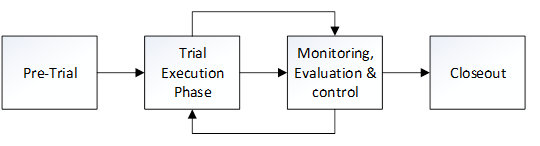
\includegraphics{images/book/pm1.png}
\caption{}
\end{figure}

\emph{Figure 5.1 Simplified temporal overview of the management process
for an intervention trial }

This module will briefly define the requirements and challenges for
project management for a clinical trial, and highlight potentially
helpful approaches and tools for each. Documentation; human subjects
concerns; development and use of a project management plan; management
of personnel and interpersonal communications; and diagnosis and
correction of problems will be discussed. For each of these, guidelines
and useful templates are provided. Given their critical importance,
activities embedded in the pre-trial phase are emphasized (see Figure
5.2).

\begin{figure}[htbp]
\centering
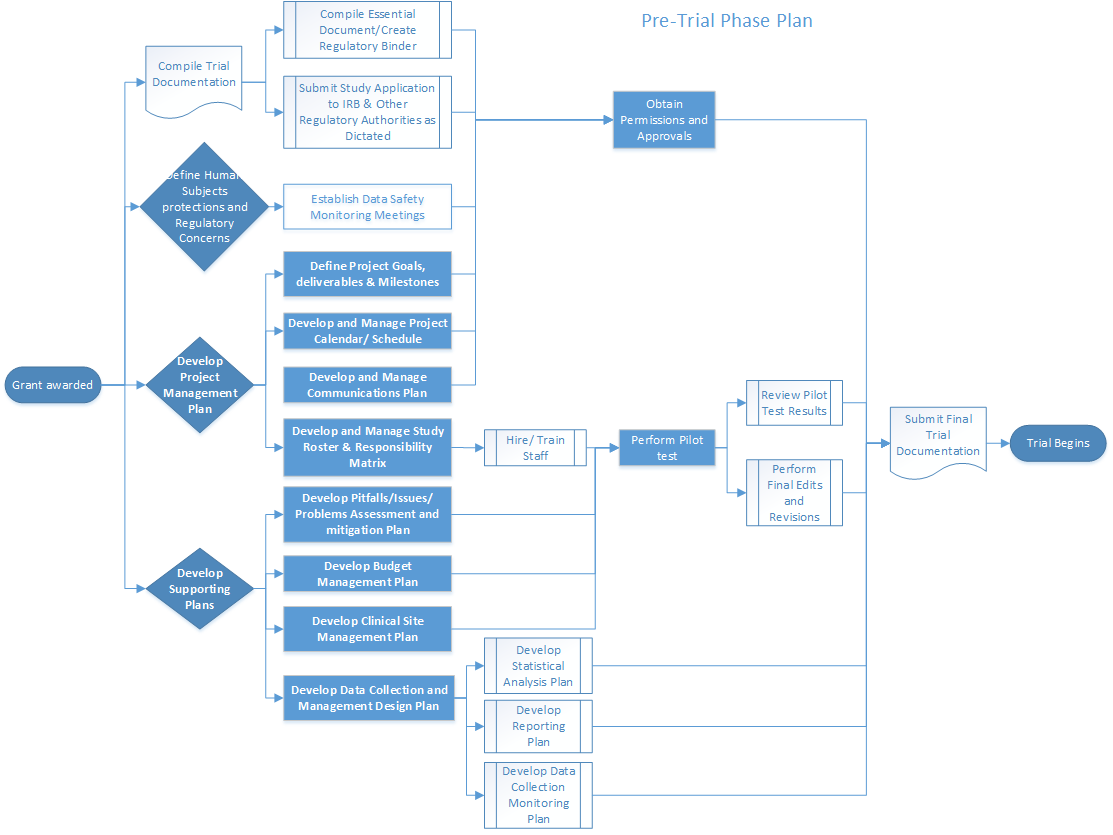
\includegraphics{images/book/pm2.png}
\caption{}
\end{figure}

\emph{Figure 5.2. Example flowchart depicting high-level summary of
Pretrial activities and their order. In bold are the activities covered
in this module. For details click on each activity relevant to each
trial phase. }

\begin{figure}[htbp]
\centering
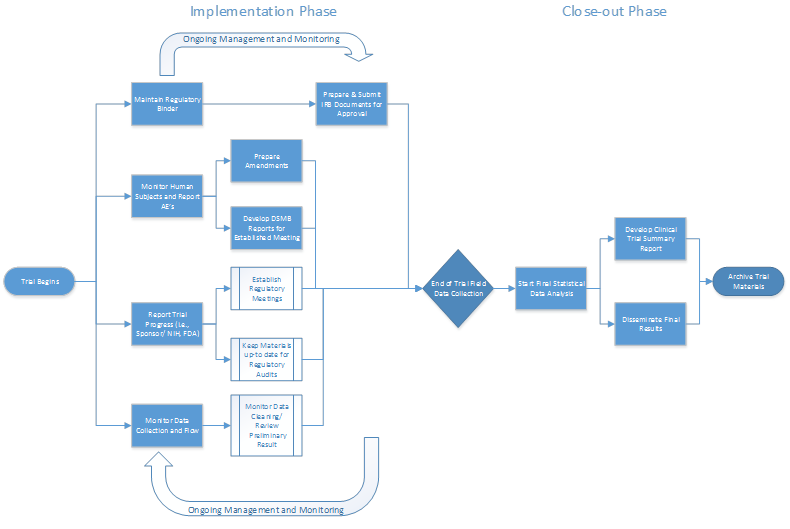
\includegraphics{images/book/pm3.png}
\caption{}
\end{figure}

\emph{Figure 5.3. Example flowchart depicting high-level summary of
trial activities }

\section{Management of trial documentation (see Essential documents
module)}\label{management-of-trial-documentation-see-essential-documents-module}

\emph{Table 5.1 Project management activities relevant for trial
documentation}

\begin{longtable}[]{@{}llll@{}}
\toprule
\begin{minipage}[b]{0.08\columnwidth}\raggedright\strut
Trial Document / Activity\strut
\end{minipage} & \begin{minipage}[b]{0.28\columnwidth}\raggedright\strut
Project Management Activities, by Phase\strut
\end{minipage} & \begin{minipage}[b]{0.35\columnwidth}\raggedright\strut
\strut
\end{minipage} & \begin{minipage}[b]{0.17\columnwidth}\raggedright\strut
\strut
\end{minipage}\tabularnewline
\midrule
\endhead
\begin{minipage}[t]{0.08\columnwidth}\raggedright\strut
\strut
\end{minipage} & \begin{minipage}[t]{0.28\columnwidth}\raggedright\strut
\textbf{Pre-trial}\strut
\end{minipage} & \begin{minipage}[t]{0.35\columnwidth}\raggedright\strut
\strut
\end{minipage} & \begin{minipage}[t]{0.17\columnwidth}\raggedright\strut
\strut
\end{minipage}\tabularnewline
\begin{minipage}[t]{0.08\columnwidth}\raggedright\strut
Regulatory Binder)\strut
\end{minipage} & \begin{minipage}[t]{0.28\columnwidth}\raggedright\strut
Set up; establish location for storage and security\strut
\end{minipage} & \begin{minipage}[t]{0.35\columnwidth}\raggedright\strut
\strut
\end{minipage} & \begin{minipage}[t]{0.17\columnwidth}\raggedright\strut
\strut
\end{minipage}\tabularnewline
\begin{minipage}[t]{0.08\columnwidth}\raggedright\strut
Protocol\strut
\end{minipage} & \begin{minipage}[t]{0.28\columnwidth}\raggedright\strut
Review and approval by relevant parties\strut
\end{minipage} & \begin{minipage}[t]{0.35\columnwidth}\raggedright\strut
\strut
\end{minipage} & \begin{minipage}[t]{0.17\columnwidth}\raggedright\strut
\strut
\end{minipage}\tabularnewline
\begin{minipage}[t]{0.08\columnwidth}\raggedright\strut
Credentials and competencies\strut
\end{minipage} & \begin{minipage}[t]{0.28\columnwidth}\raggedright\strut
Gather research team documentation (i.e., resumes, conflict of interest
forms, evidence of completion of required certifications)\strut
\end{minipage} & \begin{minipage}[t]{0.35\columnwidth}\raggedright\strut
\strut
\end{minipage} & \begin{minipage}[t]{0.17\columnwidth}\raggedright\strut
\strut
\end{minipage}\tabularnewline
\begin{minipage}[t]{0.08\columnwidth}\raggedright\strut
Investigator Brochure / Marketing\strut
\end{minipage} & \begin{minipage}[t]{0.28\columnwidth}\raggedright\strut
Develop marketing materials/ investigators brochure\strut
\end{minipage} & \begin{minipage}[t]{0.35\columnwidth}\raggedright\strut
\strut
\end{minipage} & \begin{minipage}[t]{0.17\columnwidth}\raggedright\strut
\strut
\end{minipage}\tabularnewline
\begin{minipage}[t]{0.08\columnwidth}\raggedright\strut
Manual of Procedures\strut
\end{minipage} & \begin{minipage}[t]{0.28\columnwidth}\raggedright\strut
Develop MOP; test procedures\strut
\end{minipage} & \begin{minipage}[t]{0.35\columnwidth}\raggedright\strut
\strut
\end{minipage} & \begin{minipage}[t]{0.17\columnwidth}\raggedright\strut
\strut
\end{minipage}\tabularnewline
\begin{minipage}[t]{0.08\columnwidth}\raggedright\strut
Statistical Analysis Plan\strut
\end{minipage} & \begin{minipage}[t]{0.28\columnwidth}\raggedright\strut
Review SAP; generate signoff by relevant parties\strut
\end{minipage} & \begin{minipage}[t]{0.35\columnwidth}\raggedright\strut
\strut
\end{minipage} & \begin{minipage}[t]{0.17\columnwidth}\raggedright\strut
\strut
\end{minipage}\tabularnewline
\begin{minipage}[t]{0.08\columnwidth}\raggedright\strut
Statistical Analytic Protocol\strut
\end{minipage} & \begin{minipage}[t]{0.28\columnwidth}\raggedright\strut
\strut
\end{minipage} & \begin{minipage}[t]{0.35\columnwidth}\raggedright\strut
\strut
\end{minipage} & \begin{minipage}[t]{0.17\columnwidth}\raggedright\strut
\strut
\end{minipage}\tabularnewline
\begin{minipage}[t]{0.08\columnwidth}\raggedright\strut
Data Safety and Monitoring Documents\strut
\end{minipage} & \begin{minipage}[t]{0.28\columnwidth}\raggedright\strut
Author charter; recruit DSMB members, assign chairpersonship in
partnership with funders\strut
\end{minipage} & \begin{minipage}[t]{0.35\columnwidth}\raggedright\strut
\strut
\end{minipage} & \begin{minipage}[t]{0.17\columnwidth}\raggedright\strut
\strut
\end{minipage}\tabularnewline
\begin{minipage}[t]{0.08\columnwidth}\raggedright\strut
DSMB Report\strut
\end{minipage} & \begin{minipage}[t]{0.28\columnwidth}\raggedright\strut
Develop template report; obtain relevant approvals\strut
\end{minipage} & \begin{minipage}[t]{0.35\columnwidth}\raggedright\strut
\strut
\end{minipage} & \begin{minipage}[t]{0.17\columnwidth}\raggedright\strut
\strut
\end{minipage}\tabularnewline
\begin{minipage}[t]{0.08\columnwidth}\raggedright\strut
Meeting Templates\strut
\end{minipage} & \begin{minipage}[t]{0.28\columnwidth}\raggedright\strut
Design meeting templates (agendas and minutes)\strut
\end{minipage} & \begin{minipage}[t]{0.35\columnwidth}\raggedright\strut
\strut
\end{minipage} & \begin{minipage}[t]{0.17\columnwidth}\raggedright\strut
\strut
\end{minipage}\tabularnewline
\begin{minipage}[t]{0.08\columnwidth}\raggedright\strut
Tracking /\strut
\end{minipage} & \begin{minipage}[t]{0.28\columnwidth}\raggedright\strut
Develop tracking and monitoring templates for enrollment, study visit
attendance, protocol adherence, etc.\strut
\end{minipage} & \begin{minipage}[t]{0.35\columnwidth}\raggedright\strut
\strut
\end{minipage} & \begin{minipage}[t]{0.17\columnwidth}\raggedright\strut
\strut
\end{minipage}\tabularnewline
\begin{minipage}[t]{0.08\columnwidth}\raggedright\strut
Monitoring Reports\strut
\end{minipage} & \begin{minipage}[t]{0.28\columnwidth}\raggedright\strut
\strut
\end{minipage} & \begin{minipage}[t]{0.35\columnwidth}\raggedright\strut
\strut
\end{minipage} & \begin{minipage}[t]{0.17\columnwidth}\raggedright\strut
\strut
\end{minipage}\tabularnewline
\begin{minipage}[t]{0.08\columnwidth}\raggedright\strut
Data Quality Reports\strut
\end{minipage} & \begin{minipage}[t]{0.28\columnwidth}\raggedright\strut
Develop reporting of data completeness and quality\strut
\end{minipage} & \begin{minipage}[t]{0.35\columnwidth}\raggedright\strut
\strut
\end{minipage} & \begin{minipage}[t]{0.17\columnwidth}\raggedright\strut
\strut
\end{minipage}\tabularnewline
\begin{minipage}[t]{0.08\columnwidth}\raggedright\strut
Additional Documentation\strut
\end{minipage} & \begin{minipage}[t]{0.28\columnwidth}\raggedright\strut
Develop study logs, documentation of adverse events, tracking of
participant disposition, IRB submissions and approvals, etc.\strut
\end{minipage} & \begin{minipage}[t]{0.35\columnwidth}\raggedright\strut
\strut
\end{minipage} & \begin{minipage}[t]{0.17\columnwidth}\raggedright\strut
\strut
\end{minipage}\tabularnewline
\bottomrule
\end{longtable}

\section{Management and maintenance of human subject protections and
other regualtory
interactions.}\label{management-and-maintenance-of-human-subject-protections-and-other-regualtory-interactions.}

(SEE Essential Documents Module, Human Subjects and Regulatory modules)

\section{Management of trials activities during pretrial and
execution}\label{management-of-trials-activities-during-pretrial-and-execution}

\subsection{Creating a Project Management
Plan}\label{creating-a-project-management-plan}

What

A project management plan is a document that results in a dynamic set of
documents that clearly define the goals and provide direction for the
project. It articulates the specific deliverables, as well as
procedures, timelines, and resources necessary to produce those
deliverables, as well as quality measures to meet the required
standards. The plan should be based on the scope of the project as
defined in the protocol. The following tasks are critical to creating a
project management plan:

\begin{enumerate}
\def\labelenumi{\arabic{enumi}.}
\item
  Define the project goals/deliverables/milestones
\item
  Management using outline-based and/or graphical tools for calendars
  and schedules
\item
  Management of internal and external communications
\item
  Management of project personnel and responsibilities
\end{enumerate}

Why

A well-designed project plan increases the likelihood of successfully
managing a clinical trial. It supports coherent organization, effective
management, facilitates transparency, and the detection of foreseeable
problems/ issues via monitoring of the project's critical path. The
process and subsequent documentation of all the project progress keeps
things focused and moving forward.

How

\textbf{Define project goals/ deliverables/ milestones}

The project goals, deliverables and milestones are described in the
trial protocol. The protocol should be taken as the essential and
controlling guide implicating the relevant protocol management
activities.

\textbf{Organizing structure}

Project managers should be guided by an overarching structure. For
instance, in a large and complex trial with a large number of
deliverables, investigators and managers may utilize a formal
\textbf{Work Breakdown Structure} (WBS). The WBS is a hierarchical
decomposition list of necessary tasks, with each descending level
representing an increasing detailed definition of the work. Importantly,
the WBS is designed to be focused on generation of deliverables,
i.e.~tangible work-product such as protocols, procedures and study
reports. The WBS provides a mechanism to parse deliverables into smaller
manageable components; the duration and cost of each step in the process
can thus be better established at a granular level.

For a smaller project, it may not be the case that a formal WBS is
necessary or efficient, but the \textbf{detailed breakdown of specific
tasks, along with resources required, is almost never wasted effort}.
Thus the following sections outline a system that is almost always
relevant to project management, but that may be adopted more or less
formally as circumstances dictate. The WBS can be developed using
calendaring, graphical and outlining tools.

\subsection{Management using outline-based calendars and
schedules}\label{management-using-outline-based-calendars-and-schedules}

A key component of the project's success is the management of its
schedule. The project manager should:

\begin{itemize}
\item
  Define all activities required to produce each of the project's
  deliverables.
\item
  Define the order or sequence in which the activities must happen and
  the relationship between them.
\item
  Establish the resources (both human and material) necessary to
  accomplish each activity.
\item
  Estimate the activity duration.
\end{itemize}

These items may be applied both at the high level of the project --
where, for instance, ``develop protocol'' might be a single task -- as
well as at the detailed level, where many tasks necessary to protocol
development may be broken out in detail. While the latter is a
substantial outlay of resources, it is important to note that the scope
of a task and the resources required are more easily estimated for
smaller sub-tasks. Accordingly the work invested in breaking out tasks
in detail may well be worth it in a complex project.

An example of a simplified schedule specific to protocol development is
given in Table X.3; task start and end dates, human resources, and other
materials would typically be added to this.

\emph{Table 5.3 Example of a schedule specific to protocol development}

\begin{longtable}[]{@{}l@{}}
\toprule
\begin{minipage}[t]{0.95\columnwidth}\raggedright\strut
\textbf{Activity Code} \textbf{Activity/ Deliverable} \textbf{Duration}
\textbf{Predecessor / Prerequisite}\strut
\end{minipage}\tabularnewline
\begin{minipage}[t]{0.95\columnwidth}\raggedright\strut
\textbf{(days)}\strut
\end{minipage}\tabularnewline
\bottomrule
\end{longtable}

A Draft Protocol 30 --

B Circulate Protocol Draft for Feedback and Input 14 A

C Integrate changes 18 B

D Circulate Draft Protocol for final Feedback and Input 14 C

E Finalize Protocol 8 D
---------------------------------------------------------------------------------------------------------------------------

In the above example, the activities occur in a linear fashion where one
must precede the next. Other activities and tasks may more easily and
efficiently proceed along multiple, parallel tracks.

\textbf{\emph{Management using Graphical Tools}}

Other management tools that may be helpful in creating the project
timeline or process maps include flowcharts, Gantt Charts, and network
diagrams. We present some examples of the use of these tools below.

\textbf{Flowcharts} - are graphical depictions of the process flow
corresponding to the outline format exemplified by Table 5.3. A
flowchart replicating Table 5.3 would consist of a series of boxes laid
out in boringly linear fashion and would therefore be of limited
utility. For more complex development along parallel tracks, by
contrast, a graphical depiction offers considerable advantages, as shown
in Figures 5.2 and 5.3. These flowcharts depict pretrial, execution and
closeout activities at a high level. Once again, each of the components
of the activities depicted here could itself be the subject of a
detailed tabular or graphical breakdown. A key strength of these
organizing tools is their applicability at the level of granular detail
and high-level project overview, simultaneously.

The \textbf{Network Diagram} is an enhanced flowchart that associates
each task with a duration and, potential, anticipated resource
expenditures. This is particularly useful in helping the investigative
team understand the impact of delays in any task on the overall
timeline. Because many tasks have prerequisites while others may be
worked on in parallel, it is not the case that delays in different tasks
will have similar impact.\\[2\baselineskip]A useful concept, therefore,
is the \textbf{critical path} of the project. This is defined as the
longest sequence of tasks stretching from project start to finish. It
has the feature that account for the fact that in delays in any of the
activities along the path will lead delay completion of the project,
unless this delay can be made up elsewhere along the critical path.
These concepts are illustrated in Figure 5.4.

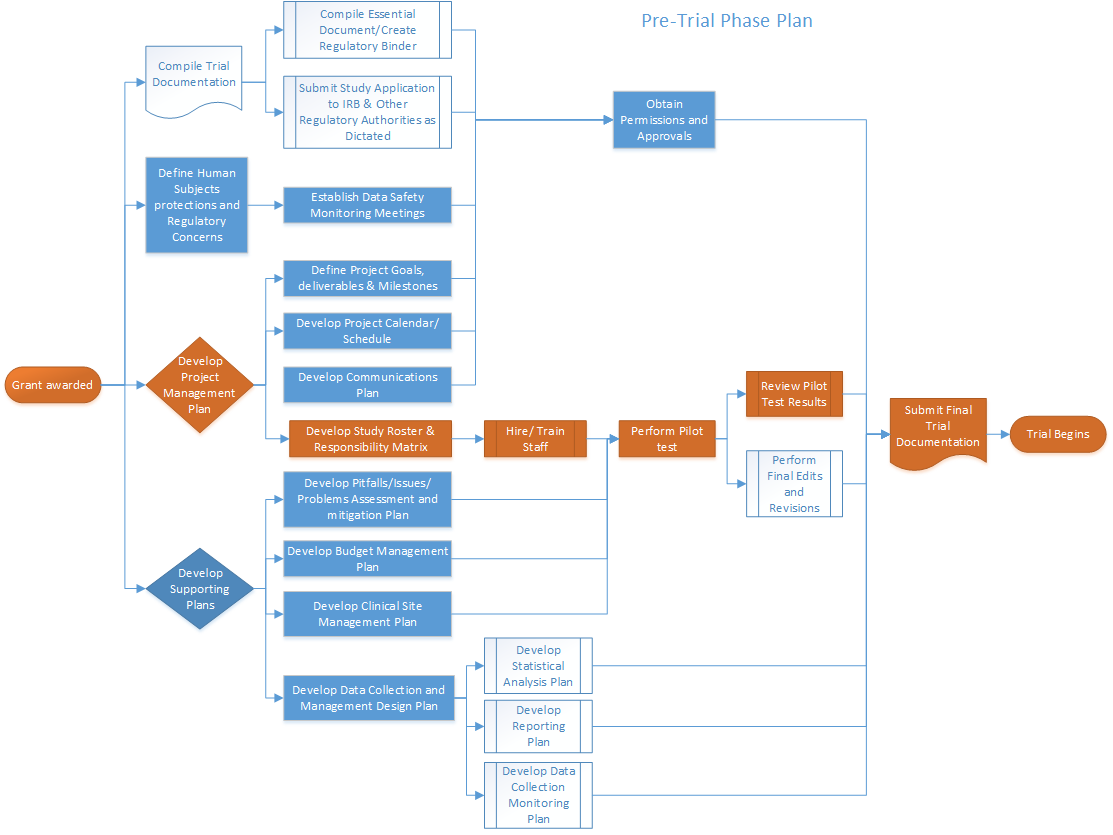
\includegraphics{images/book/pm4.png} \emph{Figure 5.4. The project
critical path is outline in orange; any delays along this path imply an
elongation of the total project duration. }

Management of internal and external communications

Key elements of the communications plan include:

\textbf{Opportunities for communication. }

The management team should assist in developing a schedule of
interactions between members of the investigative team, as well as with
internal and external stakeholders. This should include transmission of
formal reports, and also the times, locations, duration, and attendees
of meetings and other interactions.

\textbf{Means of communications.}

The management team should assist in procuring, testing and maintaining
the means of project communications. These should be chosen such that
capabilities correspond to project needs. Ease of use and reliability
are additional key features that must be emphasized.

\textbf{Recording of communications and trial progress. }

The project management team should take an active role in maintenance of
the record of communications, including meeting minutes and agendas.
Under some scenarios, stakeholders (e.g.~funding agencies) may reserve
the right to determine the official level of high-level interactions, in
which case the management team may contribute as appropriate.

\subsection{Management of project personnel and
responsibilities}\label{management-of-project-personnel-and-responsibilities}

The management team should develop a roster of personnel based on the
roles and responsibilities of team members. Ideally this will identify
the individuals primarily responsible (i.e.~those that execute the work)
and accountable (i.e.~those ultimately answerable for the completion)
for each function and task. Teams may additionally elect to identify
-those who have secondary responsibilities relating to consulting on, or
approval of, specific tasks and functions.

\section{Supporting plans}\label{supporting-plans}

\subsection{Problem assessment and mitigation management
plan}\label{problem-assessment-and-mitigation-management-plan}

Every clinical trial is subject to problems that may impact the normal
progress of the project. Fundamental to the trial's success is the
development of a comprehensive issues assessment and mitigation plan.
During the planning phase it involves the identification and
quantification of potential challenges that can impact (positively or
negatively) the trial and/or its progress. Based on the assessment, the
manager should develop a response plan. During trial phase the manager
is to monitor and control the possible issues. The purpose of a problem
assessment during the development stage of the trial is to first improve
the study design and to be able to successfully manage both the
foreseeable and unforeseeable problems.

\subsubsection{Problem Management Response
Plan}\label{problem-management-response-plan}

After identifying and evaluating potential problems that may impact the
trial, it is advisable to develop a problem management response plan.
The purpose is to develop response strategies to reduce the potential of
a problem to occur, or minimize its impact if it does. The main
components of the plan should include:

Issue management scope and objectives

The methods to identify, assess, quantify, response, monitor and control
the issue/ problem.

Personnel involved in the analysis and response processes.

The tools assigned to enhance opportunities and reduce threats to the
trial's objectives.

Issue/problem prioritization (i.e., the level of impact to the schedule,
budget and/or quality of the trial results).

A response plan for tracking identified problems, monitoring the
residual issues, identifying new problems, and evaluating issues process
effectiveness throughout the trial.

Communications plan for the distribution of problem update reports.

The key for a successful problem management plan is to maintain a
constant monitoring and reevaluation of the potential problems as well
as the circumstances in which they emerge. As problems evolve
differently during different phases of the trials it is important to be
vigilant and be adaptable.

\subsection{Clinical site management
plan}\label{clinical-site-management-plan}

Another essential element of the clinical trial's execution and its
success is the Site Management Plan. Site Management goes beyond simply
monitoring a site. It focuses on regular, consistent communication with
site stakeholders during the pre-trial, trial, and closeout phases. The
first step in the process is to identify a reliable, primary
point-of-contact for the site during the course of a trial. Is equally
vital that sites understand the importance of maintaining regular
communications with the primary study site or study Sponsor, depending
on trial type. Sites should also have a solid understanding of whom to
contact with questions, issues, and concerns that may arise at any point
during the trial.

The Site Management Plan should include a set of expectations,
organization, and the establishment of metrics to track performance, and
building and strengthen relationships. Table X.7 provides a list of
activities to undertake during the different phases of the trial.

\emph{Table 5.7 Site Management Plan during the different phases of the
Clinical Trial}

\begin{longtable}[]{@{}lll@{}}
\toprule
Pre-trial & Execution & Closeout\tabularnewline
\midrule
\endhead
Define sample size (Krishnankutty\_2012) and recruitment strategies. &
Review/ monitor data collection issues. & Complete final source data
verification of Case Report Forms (CRFs/ eCRFs), ensuring protocol
adherence, and managing the collection of final safety
data.\tabularnewline
Review site feasibility and qualifications for the study. &
&\tabularnewline
Define recruitment timeline. & &\tabularnewline
Establish Site contact/ develop relationships with sites. & Keep an
updated list of staff turnover for the sites. &\tabularnewline
Create site training and provision of study documents for the in-service
presentation (i.e., Introductory letters/ handouts/ brochures/ HIPAA
waivers). & Re-in-service sites as often as needed (to keep momentum of
the trial). &\tabularnewline
Recruit sites. & Monitor site (remotely or on-site) according to
regulations. & Ensure all documentation (regulatory correspondence) is
filed appropriately and ready for the clinical monitor or Clinical
Research Associate (CRA) to review during the close-out
visit.\tabularnewline
Follow-up site with phone calls to administrators and track those
communications in a log. & &\tabularnewline
Hire/ Train/ Develop field staff. & &\tabularnewline
Set meeting schedule for the staff. & Meet with staff weekly at first to
problem solve. Then change to bi-weekly or monthly. &\tabularnewline
Develop site monitoring/Quality Assurance log & Update log
&\tabularnewline
Define roles of study field staff vs.~sites responsibilities. &
&\tabularnewline
Inform sites on performance and contractual issues. & Track problems/
issues and their resolutions. &\tabularnewline
& & Ensure return or destruction of all study related materials (i.e.,
unused lab kits and CRFs).\tabularnewline
\bottomrule
\end{longtable}

The appropriate level of site management and oversight empowers sites to
effectively recruit, treat, and retain subjects, while ensures
regulatory compliance, protocol adherence, the protection of subjects'
right, subject safety, and overall management of screened and enrolled
subjects. Presenting a clear understanding of the communication flow
will often reduce protocol violations and deviation, an address data
issues and questions, thereby increasing the quality and integrity of
the clinical trial data.

\subsection{Budget management plan}\label{budget-management-plan}

All financial aspects of the trial must be documented in an agreement
between the sponsor and the investigator/institution. A budget
management plan should aim to monitor the budget continuously as the
trial progresses given that delays and/ or changes on the trial's scope
may negatively impact it. Scope creep or the tendency to add
requirements to the scope, often results in deliverables being out of
schedule and the trial being over budget. For this reason the budget
management plan should also include a routine schedule for revisions and
updates.

\subsection{Clinical Data Management
Plan}\label{clinical-data-management-plan}

The design of the research data lifecycle should be strategized in the
clinical data management plan (CDMP). The exact content of the CDMP will
vary on the type of trial, the number of sites involved, and the
sponsor's specifications. Among the recommended items to include are:

\begin{itemize}
\item
  Clinical data management definition and procedures

  \begin{itemize}
  \item
    Systems for data collection and management
  \item
    Data entry procedures
  \item
    Data security procedures
  \item
    Data cleaning and quality control procedures
  \item
    Data import and exports procedures
  \item
    Case Report Forms (CRF)
  \end{itemize}
\item
  Monitoring of study participants

  \begin{itemize}
  \item
    Screening/Recruitment
  \item
    Randomization/Blinding procedures
  \item
    Cessation of Intervention
  \item
    Withdrawals
  \item
    Tracking
  \end{itemize}
\item
  Reporting

  \begin{itemize}
  \item
    Safety
  \item
    Adverse events and Serious Adverse Events
  \item
    Screening and Enrollment
  \item
    Data Quality and Completeness
  \item
    Progress and Final Reports
  \item
    Additional Reports
  \end{itemize}
\item
  Trial Documents and Data Retention

  \begin{itemize}
  \item
    Retention of Trial Documents
  \item
    Data Use Agreements (DUA)
  \end{itemize}
\end{itemize}

For details see the Data management module. Other resources include
IFAR's Sensitive Data Security Policy (IFAR\_sensitive\_data\_security),
Boston Children's Hospital Guideline for Developing a Manual of
Operations (BCH\_RPG-05).

\section{Special considerations for older
subjects}\label{special-considerations-for-older-subjects-12}

None

\section{Common Pitfalls}\label{common-pitfalls-15}

Lack of management follow-up and poor communications systems.

Failure to submit amendments or keep up with study documentation
updates.

Not keeping up with staff certifications.

Personnel turnover and a lack of redundancies buildup.

Lack of compliance with regulations.

Missing reports deadlines due to a lack of organization in the calendar.

Research sites closures during the trial collection cycle.

Unanticipated scope changes that affect the budget and schedule.

Ineffective recruitment.

Ineffective mechanism to maintain blinding.

Ineffective use of technologies.

Failure to update security systems.

\chapter{Data Management}\label{data-management}

\section{Clinical Data Management}\label{clinical-data-management}

\subsection{What}\label{what-17}

Clinical Data Management (\textbf{CDM}) is the collection, cleaning, and
management of subject data in compliance with regulatory standards
(Krishnankutty\_2012). It is a critical component of clinical research.

\subsection{Why}\label{why-17}

The quality of the data generated by the clinical trial will determine
the soundness of scientific conclusions formed on the basis of analysis.

\subsection{How}\label{how-17}

Data collection and management procedures should be based on sound
statistical principles and compliant with the study protocol and
regulations. CDM protocol should address key project prerequisites
regarding the data collection, storage, protection, retention, and
reporting. Potential problems and solutions proposed solutions should be
reviewed in detail.

The International Conference On Harmonisation (ICH) Guideline E6(R2)
recommends that sponsors of clinical trials ``implement systems to
manage quality throughout the design, conduct, recording, evaluation,
reporting, and archiving of clinical trials''\ldots{} Sponsors should
focus on the ``human subject protection and reliability of trial
results''\ldots{} To warrant the quality of management ``the methods
selected to assure and control the quality of the trial need to be
proportionate to the risks inherent in the trial and the importance of
the information collected'' (E6\_R2: 5).

The NIH Intramural Research Program Guidelines section on Clinical
Informatics, Data Management, and Protocol Tracking rationale and
standard states:

\begin{quote}
\emph{``Collecting clinical data is a complex task that must be
integrated into the medical practices of the institution. To monitor the
study's progress and patient safety, data collection is best done as
data are generated. Data management organized and supported at the
institute level is more efficient and reliable than that left to the
individual investigator. There are often unforeseen uses for the kinds
of information gathered in the conduct of a clinical trial, and a
central database, with appropriate archiving, assures that this
information remains the legacy of the institute'' }

\emph{Each institute sponsoring clinical research should develop a
central clinical investigations database that maintains all data
specified to be collected in the clinical study (either intervention or
natural history). The clinical research information system being
continually developed by the Clinical Center interfaces with and
supports each institute's clinical research needs. A confederated
database will enable information exchange, enabling access to and
sharing of clinical and research information among all institutes. The
institutes require data-management infrastructures to maintain their
central data registries, to enhance existing databases, to provide
eligibility checklists, to record patient randomization and entry into
their protocols, to provide report generation, data warehousing, and
data entry forms, and to monitor data collection.'' (NIH\_standars\_CR)}

The NIA \textbf{Clinical Research Study Investigator's Toolbox} provides
guidance with specific reference to clinical trials in aging, and in
particular useful tips for data management. Investigators pursuing or
conducting federally funded projects should make use of this resource
(NIA-Guide MOP).
\end{quote}

\section{CLINICAL Data Management definition and
procedures}\label{clinical-data-management-definition-and-procedures}

\subsection{What}\label{what-18}

The clinical data management procedures define the methods and dependent
activities in which the clinical data is collected and managed. The
procedures content should include the methods used to assign and
structure participant's identifiers (ID), the location of the ID logs,
the types of data collection instruments used, a description of how the
data is captured/completed, reviewed, cleaned, and subsequently
stored/archived.

\subsection{Why}\label{why-18}

Data management procedures that are compliant with the trial's protocol,
good clinical practice (GCP), regulatory requirements, and undergo
regular process audits assures the quality of data necessary to execute
the planned analysis.

\subsection{How}\label{how-18}

The data management procedures are often incorporated as a subsection
within the Manual of Operations (MOO) or Standard Operating Procedures
(SOP). These are executed by project personnel whose portfolio of work
includes data management, and who have appropriate professional training
and credentials in data science broadly defined. IFAR encourages all
investigators and managers to author a MOO or SOP in order to document
the project operations including the data management activities
(IFAR\_sensitive\_data\_security). As noted above, the NIA toolbox
provides general guidance and specific requirements for clinical trials
conducted in the field of aging. Harvard Catalyst has a detailed
planning checklist that can assist researchers describe the data for
protection, IRB submission, and regulatory compliance
(Harvard\_Catalyst: 5).

Extensive and diverse guidance and examples in other fields are also
available online. Some well-executed examples are featured the National
Institute of Dental and Craniofacial Research (NIDCR) and Boston
Children's Hospital (BCH) Clinical Research Center websites.

\subsubsection{Systems for data collection and
management}\label{systems-for-data-collection-and-management}

Clinical trials may use paper-based or electronic data capture, with
most studies today using the latter. An electronic data capture
(\textbf{EDC}) system will be designed to facilitate data collection,
often using web-based technology. A Clinical Data Management Systems
(\textbf{CDMS}) comprises the software tools for data maintenance,
quality assurance and reporting. EDC and CDMS may be combined under a
single informatics environment.

ICH guideline E6(R2) recommends that the informatics environment allows
for both data changes (edits) and detailed trail of audits, data, and
editorial information. It also recommends maintaining an SOP for using
these systems and a security system that prevents unauthorized access to
the data (E6\_R2: 5.5).

When describing the data collection system in applications or protocols,
data management personnel should define

\begin{itemize}
\item
  \textbf{The system specifications:} the version number, security
  system, audit trail, data entry access, the annotated case report
  forms (CFR), data validation, system failure mitigation plan, and
  electronic signature features.
\item
  \textbf{User acceptance testing:} the proper function of the system.
  This includes the customized functions, validation checks, the proper
  assignment of site and/or participant identifications numbers, the
  cross confirmation of time to events variable delivery, confirmation
  of data completion, the proper functionality of electronic
  (e.g.~e-mail) alerts, as well as the proper function of role
  assignments, data exports/imports, and system reports.

  Detail concerning specific aspects of procedures governing, and design
  of, EDC and CDMS are provided in the sections below.
\end{itemize}

\paragraph{EDC/CDM systems available at
IFAR}\label{edccdm-systems-available-at-ifar}

\protect\hyperlink{systems-available-at-ifar}{See Appendix I}

\subsubsection{Data entry procedures}\label{data-entry-procedures}

These outline rules for valid data capture. They include the method for
determining that a specific form has been completed, for data cleaning
and quality assurance, storage procedures, and validation checks
designed to ensure that the data capture system operates accurately,
reliably, and consistently. With EDC, the designers of the structure may
impose rules to maintain data and study quality, ranging from the simple
(disallowing, for instance, data falsely labeled with future dates or
biological values incompatible with life) to the more complex (for
instance, implementation of automated checks of inclusion and exclusion
criteria so that ineligible individuals are not enrolled as
participants.

\subsubsection{Data Security Procedures}\label{data-security-procedures}

Procedures for maintenance of data security -- incorporating both
prevention of deletion and prevention of theft -- should follow and
expand upon the Data Safety Monitoring Plan (\textbf{DSMP}) of the study
protocol. Details on protocol development are provided in the Essential
Documents module.

These procedures should delineate pertinent risks as well as the plan
for prevention of theft or loss, including identification of the
individuals responsible for maintaining and routinely confirming data
security.

\subsection{Data cleaning and quality control
procedures}\label{data-cleaning-and-quality-control-procedures}

These describe the programmed and/or built-in procedures of the EDC
system and CDMS ensuring data validity. Again, automated procedures
(e.g.~restriction of allowable values to those that match variable
definitions) may be employed.

\subsubsection{Data import and exports
Procedures}\label{data-import-and-exports-procedures}

These detail the frequency and methods that are to be used for the
loading of data generated outside the EDC system (for instance as
measured by a third party laboratory that provides data in a flat file
external to the main trial database). Security and preservation of data
quality must be accounted for here.

\subsubsection{Case Report Forms (CRF)}\label{case-report-forms-crf}

CRF are the `source' documents -- which may be electronic forms - for
recording the protocol-required information to be reported to the
trial's sponsor on each trial subject.

Paper or electronic documents should be consistent with the source
documents (NIH\_protocol\_template). Investigator must warrant that the
case reports be accurate, complete and legible.\\[2\baselineskip]Edits
and corrections are to be documented by study personnel with initials
and dates, and be available for audits. The corrections should not
obscure, however, the original data entry such as the audit trail for
either written or electronic data corrections.

At IFAR, the design, analysis, and preparation of the interim and final
clinical trial reports should be done with the guidance of the Research
Informatics and Biostatistics cores as appropriate.

\section{Monitoring Of study
participants}\label{monitoring-of-study-participants}

Participant monitoring is a critical task for trial personnel. The CDMS
should support and facilitate this task. Some exemplary functions are
described below.

\subsection{Screening/Recruitment}\label{screeningrecruitment}

The EDC and CDMS should reinforce the inclusion/exclusion criteria such
that only eligible participants are enrolled.

\subsection{Randomization/Blinding
procedures}\label{randomizationblinding-procedures}

The EDC should facilitate assignment of participants to treatments and
control regimes in a transparent and error-free manner, while
facilitating maintenance of blinding of study personnel as appropriate.
See Experimental design and Statistical Considerations module.

\subsection{Cessation of Intervention}\label{cessation-of-intervention}

The CDMS should provide for notation and monitoring of cessation of
intervention or other trial procedures as indicated by safety
monitoring. Reason for and duration of cessation should be provided,
along with other details Note that this is distinct from withdrawal, as
described above.

\subsection{Withdrawals}\label{withdrawals}

The CDMS should facilitate the recording of participant withdrawals from
the trial. It should capture the reasons for withdrawal, relevant dates
and other details. It should also facilitate any additional contact with
participants and recording of data relevant to said contacts.

\subsubsection{Tracking}\label{tracking}

The CDMS should facilitate tracking of participants' enrollment and
progress through the trial consistent with NIH and ICH guidance and with
the reporting paradigm laid out in the Consolidated Standards of
Reporting Trials (\textbf{CONSORT}) Statement. CONSORT is a set of
recommendations for reporting the information for randomized trials
including its design, methods, results, and conclusions (Consort). It
comprises a 25-item checklist and flow diagram providing guidance for
study enrollment, retention, and monitoring as well as derivation of
analytic data sets and other data structures.

\begin{figure}[htbp]
\centering
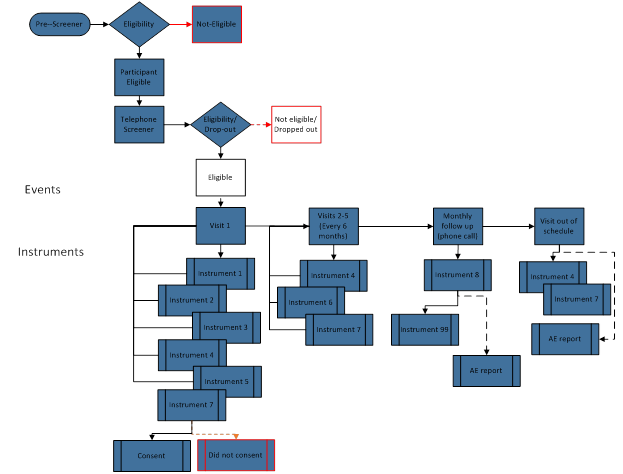
\includegraphics{images/book/dm1.png}
\caption{}
\end{figure}

Study flow diagram

\section{Reporting}\label{reporting}

A basic function of the CDMS is reporting of data and metadata relevant
to trial monitoring. Prior to the trial startup the CDM should outline
and describe the list of anticipated study reports. Some considerations
are:

\subsection{Safety}\label{safety}

Safety reports should comply with the applicable regulatory
requirement(s) and with the ICH Guidance for Clinical Safety Data
Management (FDA\_CDER\_CBER: 5.17.2). The parties that must receive the
safety reports include all concerned investigator(s)/institutions(s),
the IRB(s)/IEC(s) where required, and regulatory authorities. See Human
Subjects and Essential Documents modules for detail.

\subsubsection{Adverse events and Serious Adverse
Events.}\label{adverse-events-and-serious-adverse-events.}

The CDMS should facilitate reporting of AEs and SAEs consistent with the
study protocol and regulatory requirements (ICH\_E2A). Consideration
should be given to coding of event expectedness, severity and other
relevant qualifications. See Human Subjects and Essential Documents
modules.

\subsection{Screening and Enrollment}\label{screening-and-enrollment}

The EDC and CDMS should be constructed to facilitate regular reporting
of study progress, and specifically screening, enrollment and
participant visit tracking. A reasonable model for said reports is
contained in the DSMB reporting templates provided as part of the NIA
Toolbox
(\url{https://www.nia.nih.gov/research/dgcg/clinical-research-study-investigators-toolbox/startup}).

\subsection{Data Quality and
Completeness}\label{data-quality-and-completeness}

The EDC and CDSM should be structured to facilitate production of data
quality reporting to insure data accuracy, protocol compliance and
adherence to regulatory requirements.

\subsection{Progress and Final
Reports}\label{progress-and-final-reports}

Most federally funded projects require yearly progress and final project
reports. State usually done by the PI and grants administrator as they
require scientific and administrative progress. Again, data management
systems should be structured to interact with statistical software and
reporting to facilitate production of these reports.

\subsection{Additional Reports}\label{additional-reports}

Project-specific reporting is par for the course in any clinical trial,
and will reflect specific complexities of each design. Complex
interventions, cluster designs, and numerous other features will
necessitate redesign of standard reports or construction of new ones.
The EDC and CDMS should be structured to permit easy access to study
data and metadata for authoring of said reports within the CDMS or
parallel technology (e.g.~statistical analysis software).

\section{Trial Documents and Data
Retention}\label{trial-documents-and-data-retention}

\subsection{Retention of Trial
Documents.}\label{retention-of-trial-documents.}

Source data should be attributable, legible, contemporaneous, original,
accurate, and complete. Changes to source data should be traceable,
should not obscure the original entry and should be explained if
necessary (e.g., via an audit trail).

The ICH E6 guidance (FDA\_CDER\_CBER) recommends that trial documents be
kept by the investigator/institution as specified in Essential Documents
for the Conduct of a Clinical Trial and as required by the applicable
regulatory requirement(s). See Essential Documents module.

\subsection{Data Use Agreements (DUA)}\label{data-use-agreements-dua}

SEE Data Use Agreements in the Human Subjects and Regulatory module
(Also, IFAR\_DUA, IFAR\_sensitive\_data\_sharing).

\section{Special considerations for older
subjects}\label{special-considerations-for-older-subjects-13}

Section 164.514(a) of the Health Insurance Portability and
Accountability Act of 1996 (HIPAA) Privacy Rule provides the standard
for de-identification of protected health information, including that of
older subjects. Under this standard, health information is not
individually identifiable if it does not identify an individual and if
the covered entity has no reasonable basis to believe it can be used to
identify an individual. For older adults over 89 years of age, states
that ``all elements of dates (including year) indicative of such age,
except that such ages and elements may be aggregated into a single
category of age 90 or older'' (HHS\_hipaa).

As noted above, the NIA Toolbox is an excellent resource for guidance of
specific relevance to federal research in aging.

\section{APPENDIX I}\label{appendix-i}

\subsection{NETWORK RESOURCES}\label{network-resources}

At IFAR servers and network resources are accessible to approved staff
only. The list of IFAR preapproved network resources includes:

\begin{itemize}
\item
  IFAR file servers (e.g.~IFAR NAS)
\item
  Application servers (e.g.~REDCap, SharePoint, Accellion)
\item
  Database servers (e.g.~MySQL, SQL Server)
\item
  Application Security and User Federation
\item
  IFAR Extranet and User Repository (LDAP)
\end{itemize}

According to IFAR's sensitive data security policy projects are
encouraged to maintain a dedicated network share on IFAR or HSL
controlled file servers to ensure secure isolation of data and
materials. Investigators must also follow HSL/IFAR procedures to request
employee access to network resources (see
IFAR\_sensitive\_data\_security).

\hypertarget{systems-available-at-ifar}{\subsection{SYSTEMS AVAILABLE AT
IFAR}\label{systems-available-at-ifar}}

\subsubsection{Electronic Data Capture
(EDC)}\label{electronic-data-capture-edc}

\textbf{Research Electronic Data Capture (REDCap)} is a web application
for building and managing online surveys and databases via secure web
technologies. Each individual project in RedCap is provided a separate
workspace and the data is stored in a MySQL relational database on the
private corporate network behind several firewalls and located within
the HSL data center. The system provides features like audit trails for
tracking data entries and user activity, calendars for scheduling
events, branching logic, file uploading and calculated fields (REDCap).

\textbf{Open Clinica} is an open source clinical trial software for EDC
and CDM. The software is used to create project databases, develop
eCRFs, create validation check, schedule events, capture eCRF data from
study sites, monitor and manage the clinical data.

\subsection{Data Analytics}\label{data-analytics}

\textbf{STATA} is a statistical software package used for data analysis,
data management, graphics, simulations and custom programming for
multiple types of data (Stata). The package is available for Windows,
OS, X, and Linux. Its file format permits the exchange of data sets
between users of different operating systems (iu\_kb).

\textbf{Statistical Analysis System (SAS)} is a software package used to
enter, retrieve, and manage data. It can also retrieve data for
different operating systems to perform advance statistical and
mathematical analyses, graphics and reporting (sas).

\textbf{Statistical Package for the Social Sciences (SPSS) or IMB SPSS
Statistics} is a software used for statistical analysis, data mining,
text analytics, and data collection. Like SAS can also retrieve data
from different operating systems to perform statistical analyses,
reports, and graphics.

\textbf{R} is a language and environment for statistical computing. Its
suite of software facilities are used for data manipulation, calculation
and graphic reporting. R has the advantage to allow users to add new
programing functions.

\subsection{Reporting systems}\label{reporting-systems}

\textbf{TIBCO Jaspersoft} is an open source commercial software used in
conjunction with other open source infrastructure like MySQL and JBoss
to retrieve data, and develop reports (Swenson\_2002). The JasperReports
provides resports and analytics that can be embedded into a web or
mobile application in a variety of formats and in real-time.

(Jaspersoft).

\textbf{Shiny by RStudio} is a web application framework for R that
transforms analyses into interactive web applications (Shiny). The
application allows the manipulation of the data by sorting, filtering,
and by empowering the user to customize their analysis. At IFAR, Shiny
is used to display different project consort and compliance reports in
real time.

\textbf{JIRA} is an Atlassian software development tool used by agile
teams to plan, track, release and report Issue tracking / tasks
ticketing system.

\textbf{Google Docs} is a web-based application used to create, edit and
store documents and spreadsheets. Is part of a package offered by and
associated with \textbf{Google Apps for Business} and is compatible with
most word processor applications and presentation software
(Google\_Docs).

\textbf{Atlassian Confluence} is a team collaboration software and
enterprise wiki tool. It is used to create, organize, and discuss the
contents of projects and/or knowledge base of different IFAR centers.
The advantage of Confluence is that documents are edited in real time.

\chapter{Publication and
Dissemination}\label{publication-and-dissemination}

\section{Introduction}\label{introduction-3}

Research dissemination can be defined as follows: ``A planned process
that involves consideration of target audiences and the settings in
which research findings are to be received and, where appropriate,
communicating and interacting with wider policy and health service
audiences in ways that will facilitate research uptake in decision-
making processes and practice''. \emph{Wilson et al, Implementation
Science 2010, 5:91}

Traditionally, research dissemination centers on the publication of
results in peer reviewed journals and academic conference presentations.
Recent initiatives seek to broaden the concept of research dissemination
such that the main messages from results are communicated to targeted
decision-makers and stakeholders in a way that encourages them to factor
the research implications into their work and clinical practice. This
module will focus on two aspects of dissemination particularly relevant
to Clinical Trials: 1. Data sharing and 2. Publication in scientific
journals

Regardless of the scope, researchers are encouraged to \emph{develop a
dissemination plan early in the course of all trials.} Trials that are
closer to later phases of research translation (i.e., implementation)
and those supported by certain agencies (e.g., Patient-Centered Outcomes
Research Institute (PCORI)) may require more robust dissemination plans
in grant applications that go beyond traditional journal publications
and meeting presentations.

Resources for dissemination planning beyond journal publication:

\begin{itemize}
\item
  Agency for Healthcare Research and Quality
  \url{http://www.ahrq.gov/professionals/quality-patient-safety/patient-safety-resources/resources/advances-in-patient-safety/vol4/planningtool.html}
\item
  Communications Handbook for Clinical Trials, Chapter 6, Preparing for
  and Disseminating Study Results,
  \url{http://www.fhi360.org/sites/default/files/media/documents/CommhandbkChapterSix.pdf}
\item
  Community Alliance for Research and Engagement, Beyond a Scientific
  Publication: Strategies for Disseminating Research Findings,''
  \url{https://ctsacorus.org/resources/252/download/CARE_Dissemination_Strategies_FINAL_eversion_2.pdf}
\item
  \emph{Disseminating research findings: What should researchers do? A
  systematic scoping review of conceptual frameworks. Wilson et al,
  Implementation Science 2010, 5:91,}
  \href{http://www.ncbi.nlm.nih.gov/pmc/articles/PMC2994786/}{\emph{http://www.ncbi.nlm.nih.gov/pmc/articles/PMC2994786/}}
\end{itemize}

\section{Data Sharing}\label{data-sharing}

\subsection{What}\label{what-19}

To maximize transparency and investment, policymakers seek to expand
public and investigator access to clinical trial data. The extent of
data sharing can range from sharing aggregated data describing subject
characteristics and outcomes, to providing de-identified patient-level
data. Data sharing requirements depend on evolving policies of funding
agencies (i.e., NIH) and other regulators. \emph{Researchers are
strongly encouraged to consult the most up-to-date requirements as early
as possible in planning of their clinical trial (see section 2.3
below).}

\subsection{Why}\label{why-19}

The intent of data sharing is to maximize the transparency and benefits
of research. Moreover, some level of data sharing for clinical trials is
often required by regulatory authorities, funding agencies and the
ICMJE.

When done appropriately, data sharing:

\begin{itemize}
\tightlist
\item
  Increases public trust by increasing transparency of research efforts
\item
  Maximizes the public health impact of research
\item
  Encourages scientific inquiry and new research efforts
\item
  Encourages diversity of analysis and opinion
\item
  Permits the creation of new datasets when data from multiple sources
  are combined
\end{itemize}

\subsection{How}\label{how-19}

In September 2016 the Department of Health and Human Services (HHS)
issued a new regulation and the NIH has issued a new policy to increase
the availability of information about clinical trials.~ The HHS
\href{https://www.federalregister.gov/documents/2016/09/21/2016-22129/clinical-trials-registration-and-results-information-submission}{Final
Rule} describes requirements for registering and submitting summary
results information for certain clinical trials to
\href{file:///C:/Users/elainebergman/AppData/Local/Microsoft/Windows/Temporary\%20Internet\%20Files/Content.Outlook/SJPDZYVY/ClinicalTrials.gov}{ClinicalTrials.gov}.~
A complimentary
\href{https://www.federalregister.gov/documents/2016/09/21/2016-22379/dissemination-of-nih-funded-clinical-trial-information}{NIH
policy} that applies to all clinical trials funded by NIH, regardless of
whether they are subject to the Final Rule was also published today. The
Final NIH Policy was also published in the
\href{http://grants.nih.gov/grants/guide/notice-files/NOT-OD-16-149.html}{NIH
Guide for Grants and Contracts}.

NIH has made available the following resources to help explain these
changes.~

\begin{itemize}
\item
  \href{https://www.nih.gov/news-events/summary-hhs-nih-initiatives-enhance-availability-clinical-trial-information}{A
  summary of the Final Rule and NIH policy}
\item
  \href{https://www.nih.gov/news-events/summary-table-hhs-nih-initiatives-enhance-availability-clinical-trial-information}{A
  table of the key elements of the Final Rule and NIH policy}
\item
  \href{https://prsinfo.clinicaltrials.gov/FinalRuleChanges-16Sept2016.pdf}{A
  summary table of changes from current practice described in the Final
  Rule}
\end{itemize}

\subsubsection{Methods for Data Sharing}\label{methods-for-data-sharing}

There are numerous approaches to data sharing, each of which has
different levels of privacy protection and mechanisms for sharing.
Researchers can manage requests for data personally on an individual
request basis, or through use of a secure data archive or enclave.
Investigators should select a mode of data sharing that is appropriate
based on the size, complexity and sensitivity of the data, as well as
the volume of data use requests anticipated. See the
\href{http://grants.nih.gov/grants/policy/data_sharing/data_sharing_guidance.htm\#methods}{NIH
data sharing guidance} for details.

The NIH provides numerous
\href{https://www.nlm.nih.gov/NIHbmic/nih_data_sharing_repositories.html}{data
sharing repositories} which make data accessible for reuse. If you are
doing an NIH funded trial, consult your Project Officer to discuss
options for sharing data.

IFAR has created several sensitive data policies (including data access,
encryption, sharing, security, suppression, retention and destruction,
etc.) please see these policies on the
\href{http://thehslhub/Departments/Roslindale/HSL-IFAR/Administration/Policies-and-Forms}{HSL
HUB policy and forms}.

\subsubsection{Human Subjects and Privacy
Issues}\label{human-subjects-and-privacy-issues}

All data sharing activities must be compliant with HIPAA, local, state
and organizational regulations. All compliances and restrictions should
be addressed in the data sharing plan section of the funding
application. There are two basic approaches to protecting sensitive
data: restricting information in the shared dataset, and restricting
access to the data. See
\href{file:////hebrewseniorlife.local/home/research-users/ElaineBergman/ISAC/Data\%20Sharing\%20Publication\%20and\%20dissemination}{NIH
data sharing guidance}
(\url{http://grants.nih.gov/grants/policy/data_sharing/data_sharing_guidance.htm\#methods})
for details.

The plan for data sharing may include stripping a dataset of all
potential participant identifiers. Depending on the data and study
population, the level of information that will need to be removed from
the database varies. Studies involving participants with unusual
characteristics (Samples drawn from small geographic areas, rare
populations, and linked datasets) will likely involve a greater degree
of anonymizing to ensure the privacy of study participants.

Data archives and enclaves can be set up to restrict access at any
level. Data Use Agreements restrict the use of data to those
specifically identified in the agreement, and require that data be used
only for research purposes.

Please see the
\href{http://thehslhub/Departments/Roslindale/HSL-IFAR/Administration/Policies-and-Forms}{IFAR
policy on Limited Data Sets and Data Use agreements} on the HSL HUB as
well as the
\href{http://thehslhub/Forms/Documents-and-Forms/IFAR/IFAR-IRB-SOP}{HSL
IRB SOPs on HIPAA and the use of data in research}.

\subsection{Special considerations for older
subjects}\label{special-considerations-for-older-subjects-14}

NONE

\subsection{Common Pitfalls}\label{common-pitfalls-16}

\begin{itemize}
\tightlist
\item
  Not being aware of and planning for up-to-date data sharing
  requirements by funding agencies, regulators, and ICMJE
\item
  Failure to develop a clear well documented dataset can undermine the
  researchers ability to share the data or others to use it.
\item
  Failure to plan for the time and expense of data sharing
\end{itemize}

\subsection{Resources}\label{resources-17}

External:

\begin{itemize}
\item
  NIH Data Sharing Policy and resource page
  \href{http://grants.nih.gov/grants/guide/notice-files/NOT-OD-16-149.html}{NIH
  Guide for Grants and Contracts}.

  \begin{itemize}
  \tightlist
  \item
    \href{https://www.nih.gov/news-events/summary-hhs-nih-initiatives-enhance-availability-clinical-trial-information}{A
    summary of the Final Rule and NIH policy}
  \item
    \href{https://www.nih.gov/news-events/summary-table-hhs-nih-initiatives-enhance-availability-clinical-trial-information}{A
    table of the key elements of the Final Rule and NIH policy}
  \item
    \href{https://prsinfo.clinicaltrials.gov/FinalRuleChanges-16Sept2016.pdf}{A
    summary table of changes from current practice described in the
    Final Rule}
  \end{itemize}
\item
  Clinicaltrials.gov, \url{https://clinicaltrials.gov/}
\end{itemize}

Hebrew Senior Life:

\begin{itemize}
\tightlist
\item
  HSL IFAR Data Policies
  \url{http://thehslhub/Departments/Roslindale/HSL-IFAR/Administration/Policies-and-Forms}
\item
  HSL IRB Policies and Procedures
  \url{http://thehslhub/Forms/Documents-and-Forms/IFAR/IFAR-IRB-SOP}
\end{itemize}

\section{Scientific Publications and
Presentations}\label{scientific-publications-and-presentations}

\subsection{General Considerations}\label{general-considerations-1}

All paper and abstracts emanating from your trial should be planned
early on in the study to maximize the productivity from the trial and
avoid iterative papers. In planning, it is useful to outline the topic
of paper, target journal and responsible first author.

Larger trials should have a \emph{Publications Steering Committee} whose
members are usually the lead investigators and establish written
guidelines for vetting papers emanating from the trial. This procedure
for planning, reviewing and approving all scientific publications
(papers and abstracts) prior to submission to ensure they are accurate
(i.e., align with protocol), not duplicative, and respect ICMJE
authorship guidelines. Certain funding agencies and industry sponsors
trials may have very specific requirements regarding their own review
and approval of manuscripts prior to submission.

Section III of the
\href{https://www.acrin.org/RESEARCHERS/POLICIES/PUBLICATIONSPOLICY/PUBLICATIONSPOLICYDOCUMENT.aspx}{ACRIN
publication policy} provides details related to the roles and
responsibilities of publication committees.

\subsection{Specific Reporting Guidelines for Clinical
Trials}\label{specific-reporting-guidelines-for-clinical-trials}

Clinical trials reporting has specific standard guidelines that differ
by the type of trial design and which are continually being updated. For
example, there are set standards for the flow diagrams presenting
subject participation in a clinical trial that differ between
traditional parallel design randomized trials, non-inferiority trials,
cluster randomized trials, stepped wedge designs etc. Journals generally
follow the guidelines described in the
\href{http://www.consort-statement.org/}{\textbf{CONSORT} (Consolidated
Standards of Reporting Trials) statement}.

The \href{http://www.equator-network.org/}{EQUATOR} (Enhancing the
QUAlity and Transparency Of health Research) is also a very useful
comprehensible searchable website with up-to-date links the CONSORT
statements and extensions.

\subsection{Publication of the trial
protocol}\label{publication-of-the-trial-protocol}

\subsubsection{What}\label{what-20}

Protocol manuscripts report the methodology of your clinical trial.
Details in a published protocol paper (e.g., primary and secondary
outcome definitions, sample size estimates) need to align with other
official communications describing the study's methodology such as the
trial protocol and descriptions in ClinicalTrials.gov. These documents
may be compared by journals considering publication of the trial's
results and discrepancies will need to be explained.

\subsubsection{Why}\label{why-20}

Reasons to publish a protocol paper include increasing transparency of
the trial conduct, providing a detailed reference for future
publications emanating from the study, and demonstrating productivity
for funding agencies.

\subsubsection{How}\label{how-20}

Planning for a protocol manuscript submission should begin early because
journals generally only consider publishing protocol papers for studies
that have received ethics approval but have not yet concluded patient
recruitment.

\subsubsection{Selecting a Journal}\label{selecting-a-journal}

Examples of journals that publish protocol papers include: Clinical
Trials: Journal of the Society of Clinical Trials, Contemporary Clinical
Trials, International Journal of Clinical Trials, Journal of Clinical
Trials, BMJ, and Trials. Some of these journal allow authors to pay for
publication of their protocol paper (e.g., Journal of Clinical Trials)
and others have the option of paying for open access should the paper be
accepted.

In deciding which journal is the most appropriate to publish your
protocol, it is useful to first review prior protocol papers published
in specific journals to see which best aligns with your study and
examine their formats. All journals will have specific guidelines for
preparation which should be carefully consulted and adhered to.

\subsection{Publication of the results of a clinical
trial}\label{publication-of-the-results-of-a-clinical-trial}

\subsubsection{Timing}\label{timing}

The \href{http://www.who.int/ictrp/results/reporting/en/}{WHO Statement
on Public Disclosure of Clinical Trial Results} states, at a minimum,
main findings of clinical trials, positive or negative, are to be
submitted for publication in a peer reviewed journal within 12 months of
study completion and are to be published through an open access
mechanism unless there is a specific reason why open access cannot be
used, or otherwise made available publicly at most within 24 months of
study completion.

\subsubsection{Trial Registration
Identification}\label{trial-registration-identification}

As per the
\href{http://www.icmje.org/recommendations/browse/manuscript-preparation/preparing-for-submission.html}{ICMJE
guidelines}, top-tier journals require that your trial be registered on
\href{https://clinicaltrials.gov/}{ClinicalTrials.gov}
(\url{https://clinicaltrials.gov/}) (or equivalent such as
\href{http://www.who.int/ictrp/network/primary/en/index.html}{WHO
International Clinical Trials Registry Platform (ICTRP)}) prior to the
enrollment of the first subject, otherwise the paper will be rejected
without review. The trial registration number must be included in your
manuscript and usually appears at the end of the abstract.

The ICMJE encourages posting of clinical trial results in clinical trial
registries. The ICMJE will not consider as prior publication the posting
of trial results in any registry that meets the above criteria if
results are limited to a brief (500 word) structured abstract or tables
(to include patients enrolled, key outcomes, and adverse events).

\subsubsection{Packaging results}\label{packaging-results}

Investigators are cautioned to carefully plan the paper (s) emanating
from a single trial to avoid iterative publications, ensure the main
trial results are not usurped by early papers, and to adhere with the
pre-specified analyses set forth in the trial protocol and as described
on ClinicalTrials.gov. One should reserve the main paper to include the
pre-specified primary and secondary outcomes. \emph{``Outcome
switching'' (i.e., changing the outcomes reported in results paper with
those pre-specified in the protocol and on ClinicalTrials.gov) must be
avoided.}

Following publication of the main paper, non-iterative auxiliary papers
that leverage the rich clinical trials data may be considered.

\subsubsection{Manuscript Preparation}\label{manuscript-preparation}

All manuscripts should adhere to the guidelines provided in each
journals' Instructions for Authors which generally follow
\href{http://www.icmje.org/recommendations/browse/manuscript-preparation/preparing-for-submission.html}{ICMJE
guidelines}
(\url{http://www.icmje.org/recommendations/browse/manuscript-preparation/preparing-for-submission.html})

Most journals which have a specific reporting criteria for clinical
trials results manuscripts which generally follow the
\href{http://www.consort-statement.org/}{CONSORT statement}
(\url{http://www.consort-statement.org/}). CONSORT provides an extremely
useful
\href{http://www.consort-statement.org/checklists/view/32-consort/66-title}{checklist}
(\url{http://www.consort-statement.org/checklists/view/32-consort/66-title})
to help guide presentation of every element of a clinical trial
manuscript and is a \textbf{\emph{highly recommended resource.}}

\subsubsection{Adjunct material}\label{adjunct-material}

Most top tier journals will request a copy of the trial protocol with
the submission of the paper describing the clinical trial results.
Editors will compare the details in the protocol, ClinicalTrials.gov and
any previously published protocol papers, with those described in the
submitted manuscript to ensure they align.

\subsection{Special considerations for older
subjects}\label{special-considerations-for-older-subjects-15}

NONE

\subsection{Common Pitfalls}\label{common-pitfalls-17}

\begin{itemize}
\tightlist
\item
  Failure to develop a publication plan and committee early in the
  course of the trial.
\item
  Failure to register the trial on ClinicalTrials.gov prior to
  enrollment of the first subject.
\item
  Failure to submit trial results for publication within 12 months of
  trial completion and failure to publish results within 24 months.
\item
  Failure to follow ICMJE, journal specific, and CONSORT guidelines for
  preparing clinical trials publications.
\item
  Failure to align details of the trial in submitted papers to details
  as described in the protocol and on ClinicalTrials.gov, particularly
  pre-specified primary and secondary outcomes
\item
  Publishing iterative papers or early papers that usurp publication of
  main findings.
\item
  Missing opportunities for results dissemination beyond peer reviewed
  journals and professional conferences.
\end{itemize}

\subsection{Resources}\label{resources-18}

\begin{itemize}
\tightlist
\item
  American College of Radiology Imaging Network Publications Policy,
  \url{https://www.acrin.org/RESEARCHERS/POLICIES/PUBLICATIONSPOLICY/PUBLICATIONSPOLICYDOCUMENT.aspx}
\item
  Author's Submission Toolkit: A Practical Guide to getting your
  research Published, Current Medical Research \& Opinion Vol 26, No 8,
  2010 1967-1982.
  \url{http://www.ismpp.org/assets/docs/Certification/StudyMaterials/patel\%20m\%202010.pdf}
\item
  CONSORT (Consolidated Standards of Reporting Trials) statement
  \url{http://www.consort-statement.org/}
\item
  Equator Network Essential resources for writing and publishing health
  research, \url{http://www.equator-network.org/}
\item
  General ICMJE guidelines for preparing manuscripts for publication in
  scientific journals
  \url{http://www.icmje.org/recommendations/browse/manuscript-preparation/preparing-for-submission.html}
\item
  WHO statement on timing of clinical trials results
  \url{http://www.who.int/ictrp/results/reporting/en/}
\end{itemize}

\end{document}
